% !TEX root = ../main.tex
\section{实验配置与完整结果}

\subsection{主要训练超参数}

表\ref{tab:hyperparams}给出两个阶段的主要超参数。
已知与未知拓扑阶段的训练预算明显不同，因此正文只比较误差量级，
不进行严格的阶段间性能排名。

\begin{table}[H]
  \centering
  \caption{已知拓扑 phase4 与未知拓扑 phase6 的主要训练配置。}
  \label{tab:hyperparams}
  \begin{tabularx}{0.95\textwidth}{@{}l>{\raggedright\arraybackslash}X>{\raggedright\arraybackslash}X@{}}
    \toprule
    配置 & 已知拓扑 phase4 & 未知拓扑 phase6 \\
    \midrule
    训练轮数 & 30 & 100 \\
    隐藏维数 & 64 & 64 \\
    批量大小 & 32 & 64 \\
    学习率 & 0.01 & 学习器 0.001；生成器 0.05 \\
    优化器 & Adam & Adam \\
    dropout & 0.2 & 未使用 \\
    训练 seed & 21 & 7、21、42 \\
    数据 seed & 21 & 21（固定缓存） \\
    温度 & 不适用 & 指数退火 3.0 $\to$ 0.1 \\
    每轮学习器更新 & 全训练集 1 轮 & 固定硬图，全训练集 3 轮 \\
    每轮生成器更新 & 不适用 & 软图 20 批 \\
    正则 & 无 & 熵正则 $\lambda=0.005$ \\
    样本策略 & 原始训练集 & 四层无放回配额 300/2700/1800/1200 \\
    \bottomrule
  \end{tabularx}
\end{table}

\subsection{未知拓扑全部训练随机种子}

表\ref{tab:all-seeds}列出 9 次结构学习运行。
最低验证 CE 规则选中 ER seed 42、WS seed 7 和 BA seed 7。
ER seed 7 与 BA seed 21 的 TPR 均为 1，
但 Precision 很低，
说明模型几乎把所有真实边包含在一个严重过密的预测图中；
只报告 TPR 会掩盖这一失败模式。

\begin{table}[H]
  \centering
  \caption{未知拓扑阶段全部 9 次运行。
星号表示该网络最终选中的 seed。}
  \label{tab:all-seeds}
  \begin{tabular}{@{}lrrrrrrr@{}}
    \toprule
    网络 & seed & 验证 CE & ACC & Precision & F1 & TPR & 预测/真实边数 \\
    \midrule
    ER & 7  & 0.078580 & 0.5063 & 0.1729 & 0.2949 & 1.0000 & 2955/511 \\
    ER & 21 & 0.073931 & 0.9851 & 0.9009 & 0.9299 & 0.9609 & 545/511 \\
    ER & 42$^*$ & 0.073868 & 0.9869 & 0.9223 & 0.9374 & 0.9530 & 528/511 \\
    WS & 7$^*$ & 0.074515 & 1.0000 & 1.0000 & 1.0000 & 1.0000 & 300/300 \\
    WS & 21 & 0.076552 & 0.9818 & 0.7692 & 0.8696 & 1.0000 & 390/300 \\
    WS & 42 & 0.074528 & 0.9998 & 0.9967 & 0.9983 & 1.0000 & 301/300 \\
    BA & 7$^*$ & 0.074649 & 0.9992 & 0.9864 & 0.9932 & 1.0000 & 295/291 \\
    BA & 21 & 0.081632 & 0.1323 & 0.0635 & 0.1193 & 1.0000 & 4586/291 \\
    BA & 42 & 0.074818 & 0.9984 & 0.9764 & 0.9864 & 0.9966 & 297/291 \\
    \bottomrule
  \end{tabular}
\end{table}

\subsection{已知拓扑完整六面板诊断}

图\ref{fig:appendix-known-overview}给出 ER、WS、BA 三类网络的完整六面板诊断，用于核查正文压缩图中未展开的分桶恢复率、$\Delta\gamma$ 和初始感染人数敏感性。
由于每张图信息密度较高，
统一置于横向附录页。

\begin{landscape}
\begin{figure}[p]
  \centering
  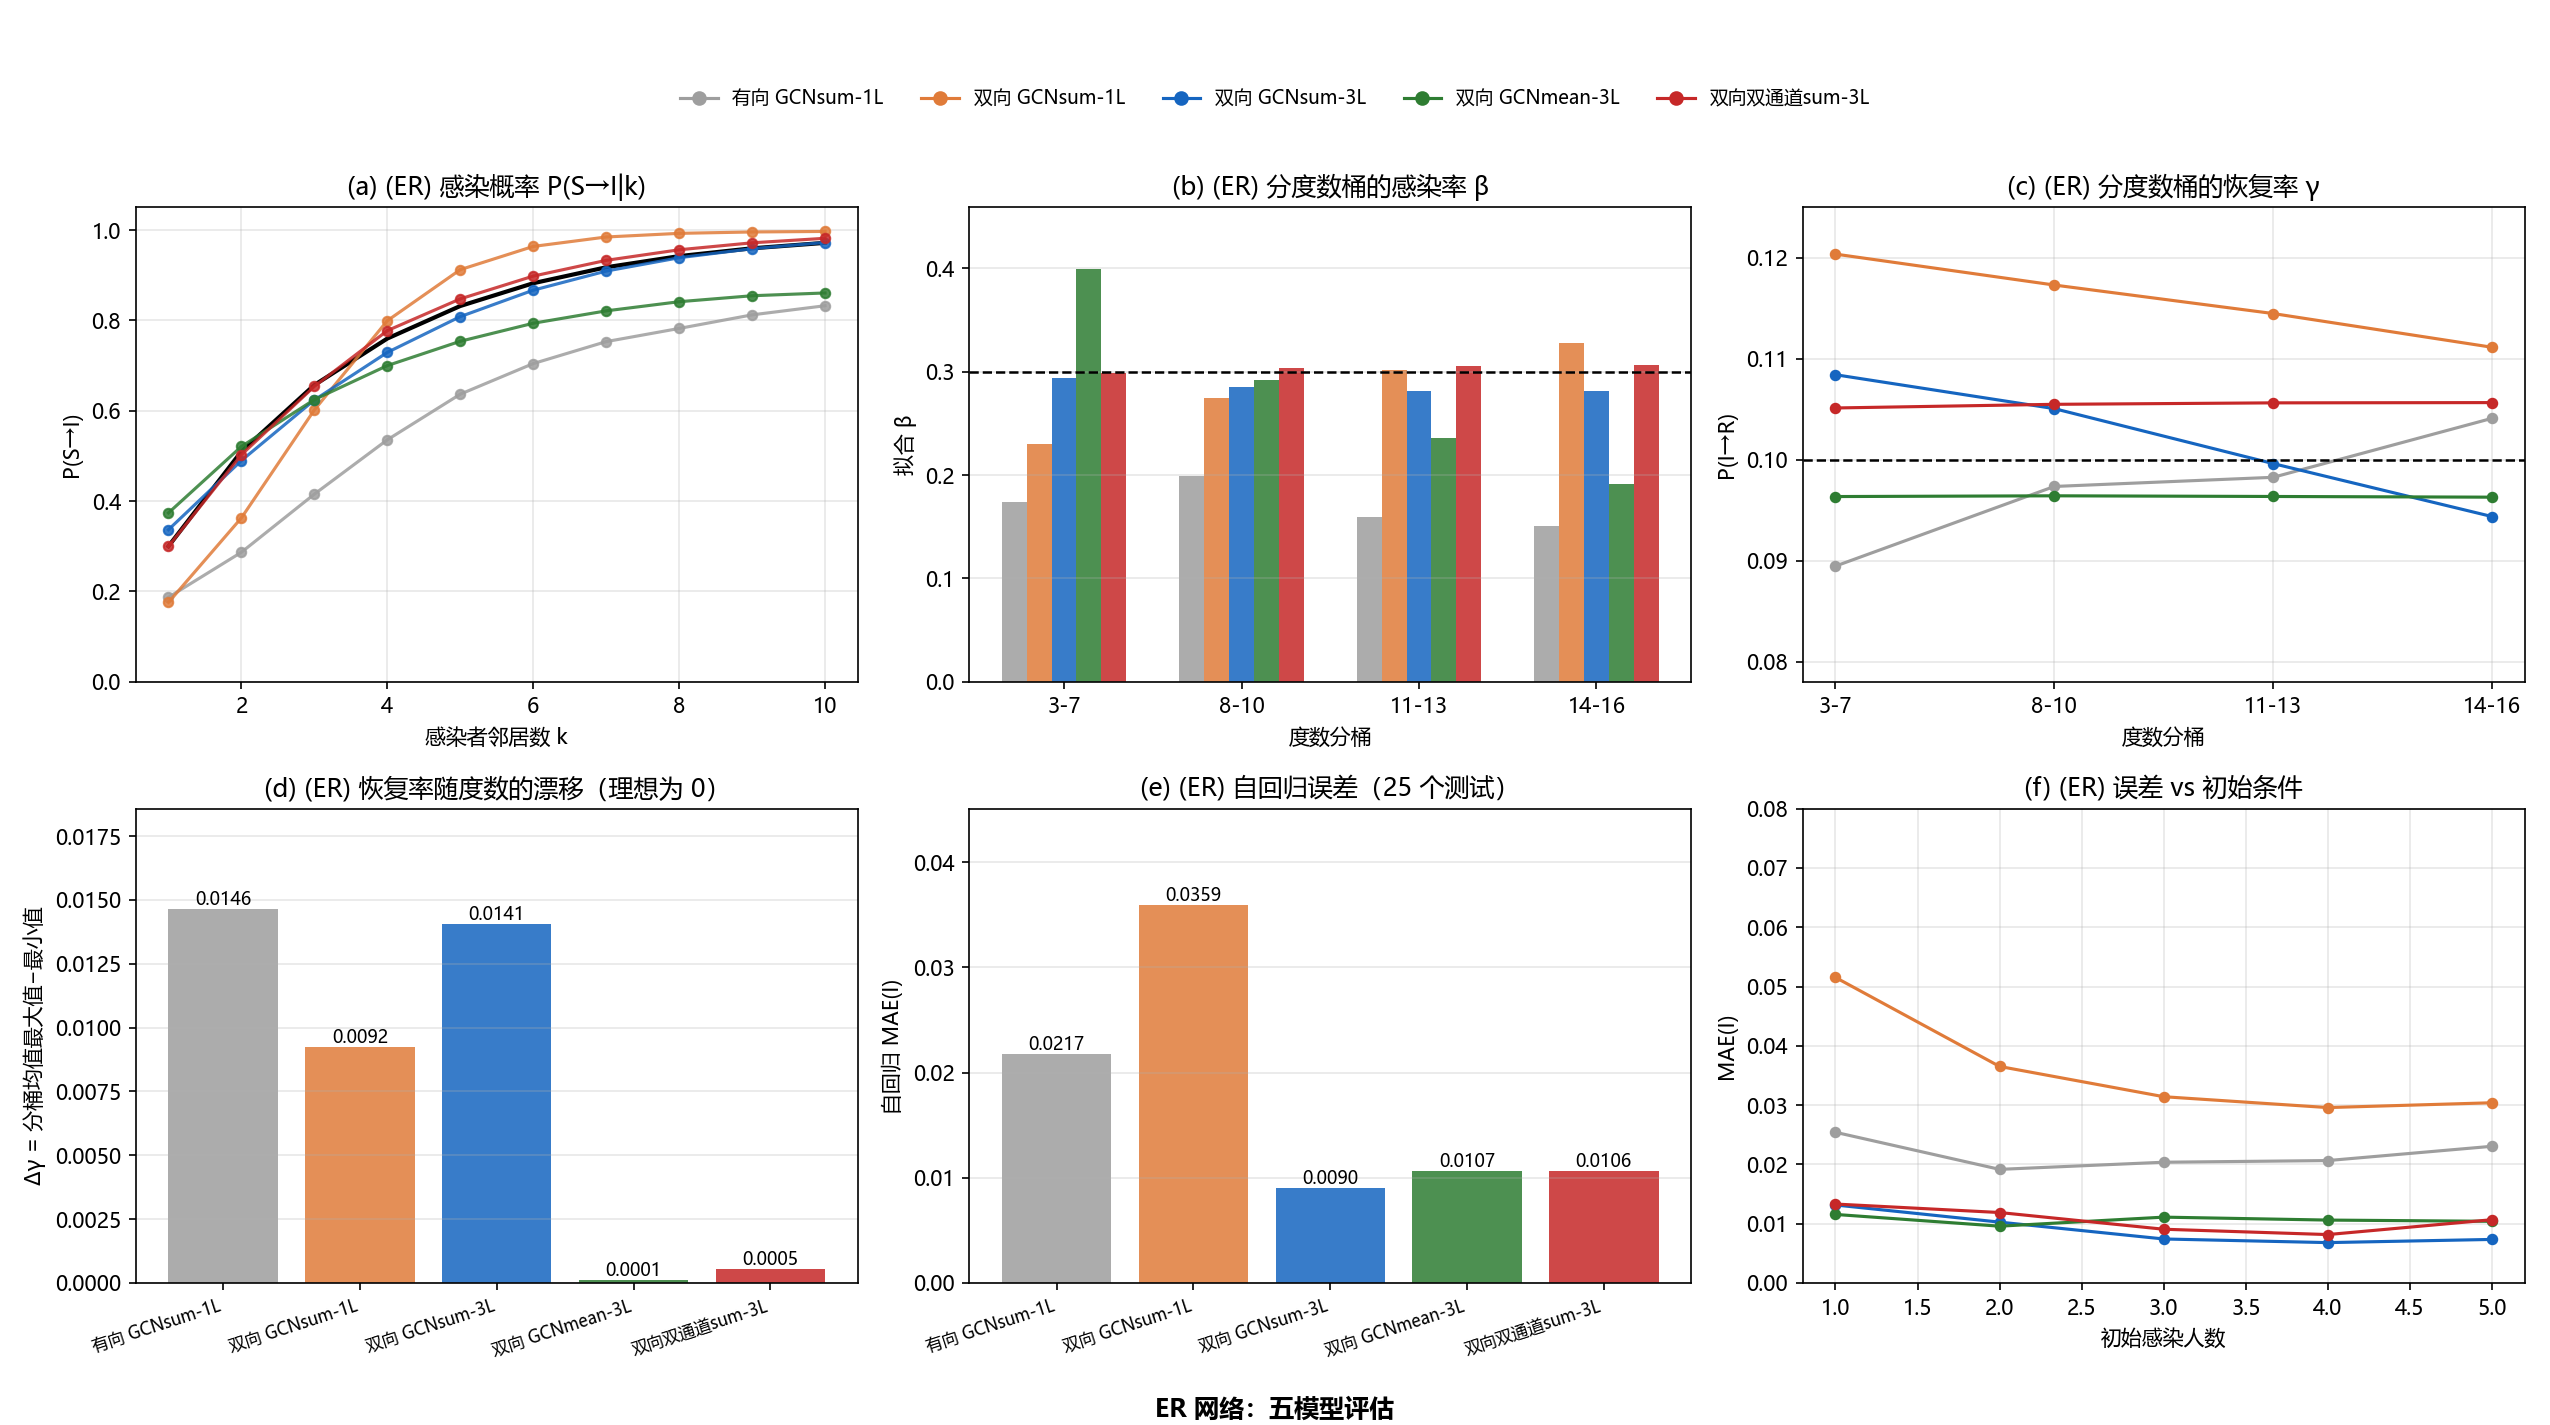
\includegraphics[width=0.96\linewidth]{fig_overview_ER.png}
  \caption{已知拓扑：ER 网络五模型完整诊断。
图中模型名称沿用 phase4 结果文件；
正文将 \code{twob3l\_bi} 统一称为双向双通道模型。}
  \label{fig:appendix-known-overview}
\end{figure}
\end{landscape}

\begin{landscape}
\begin{figure}[p]
  \centering
  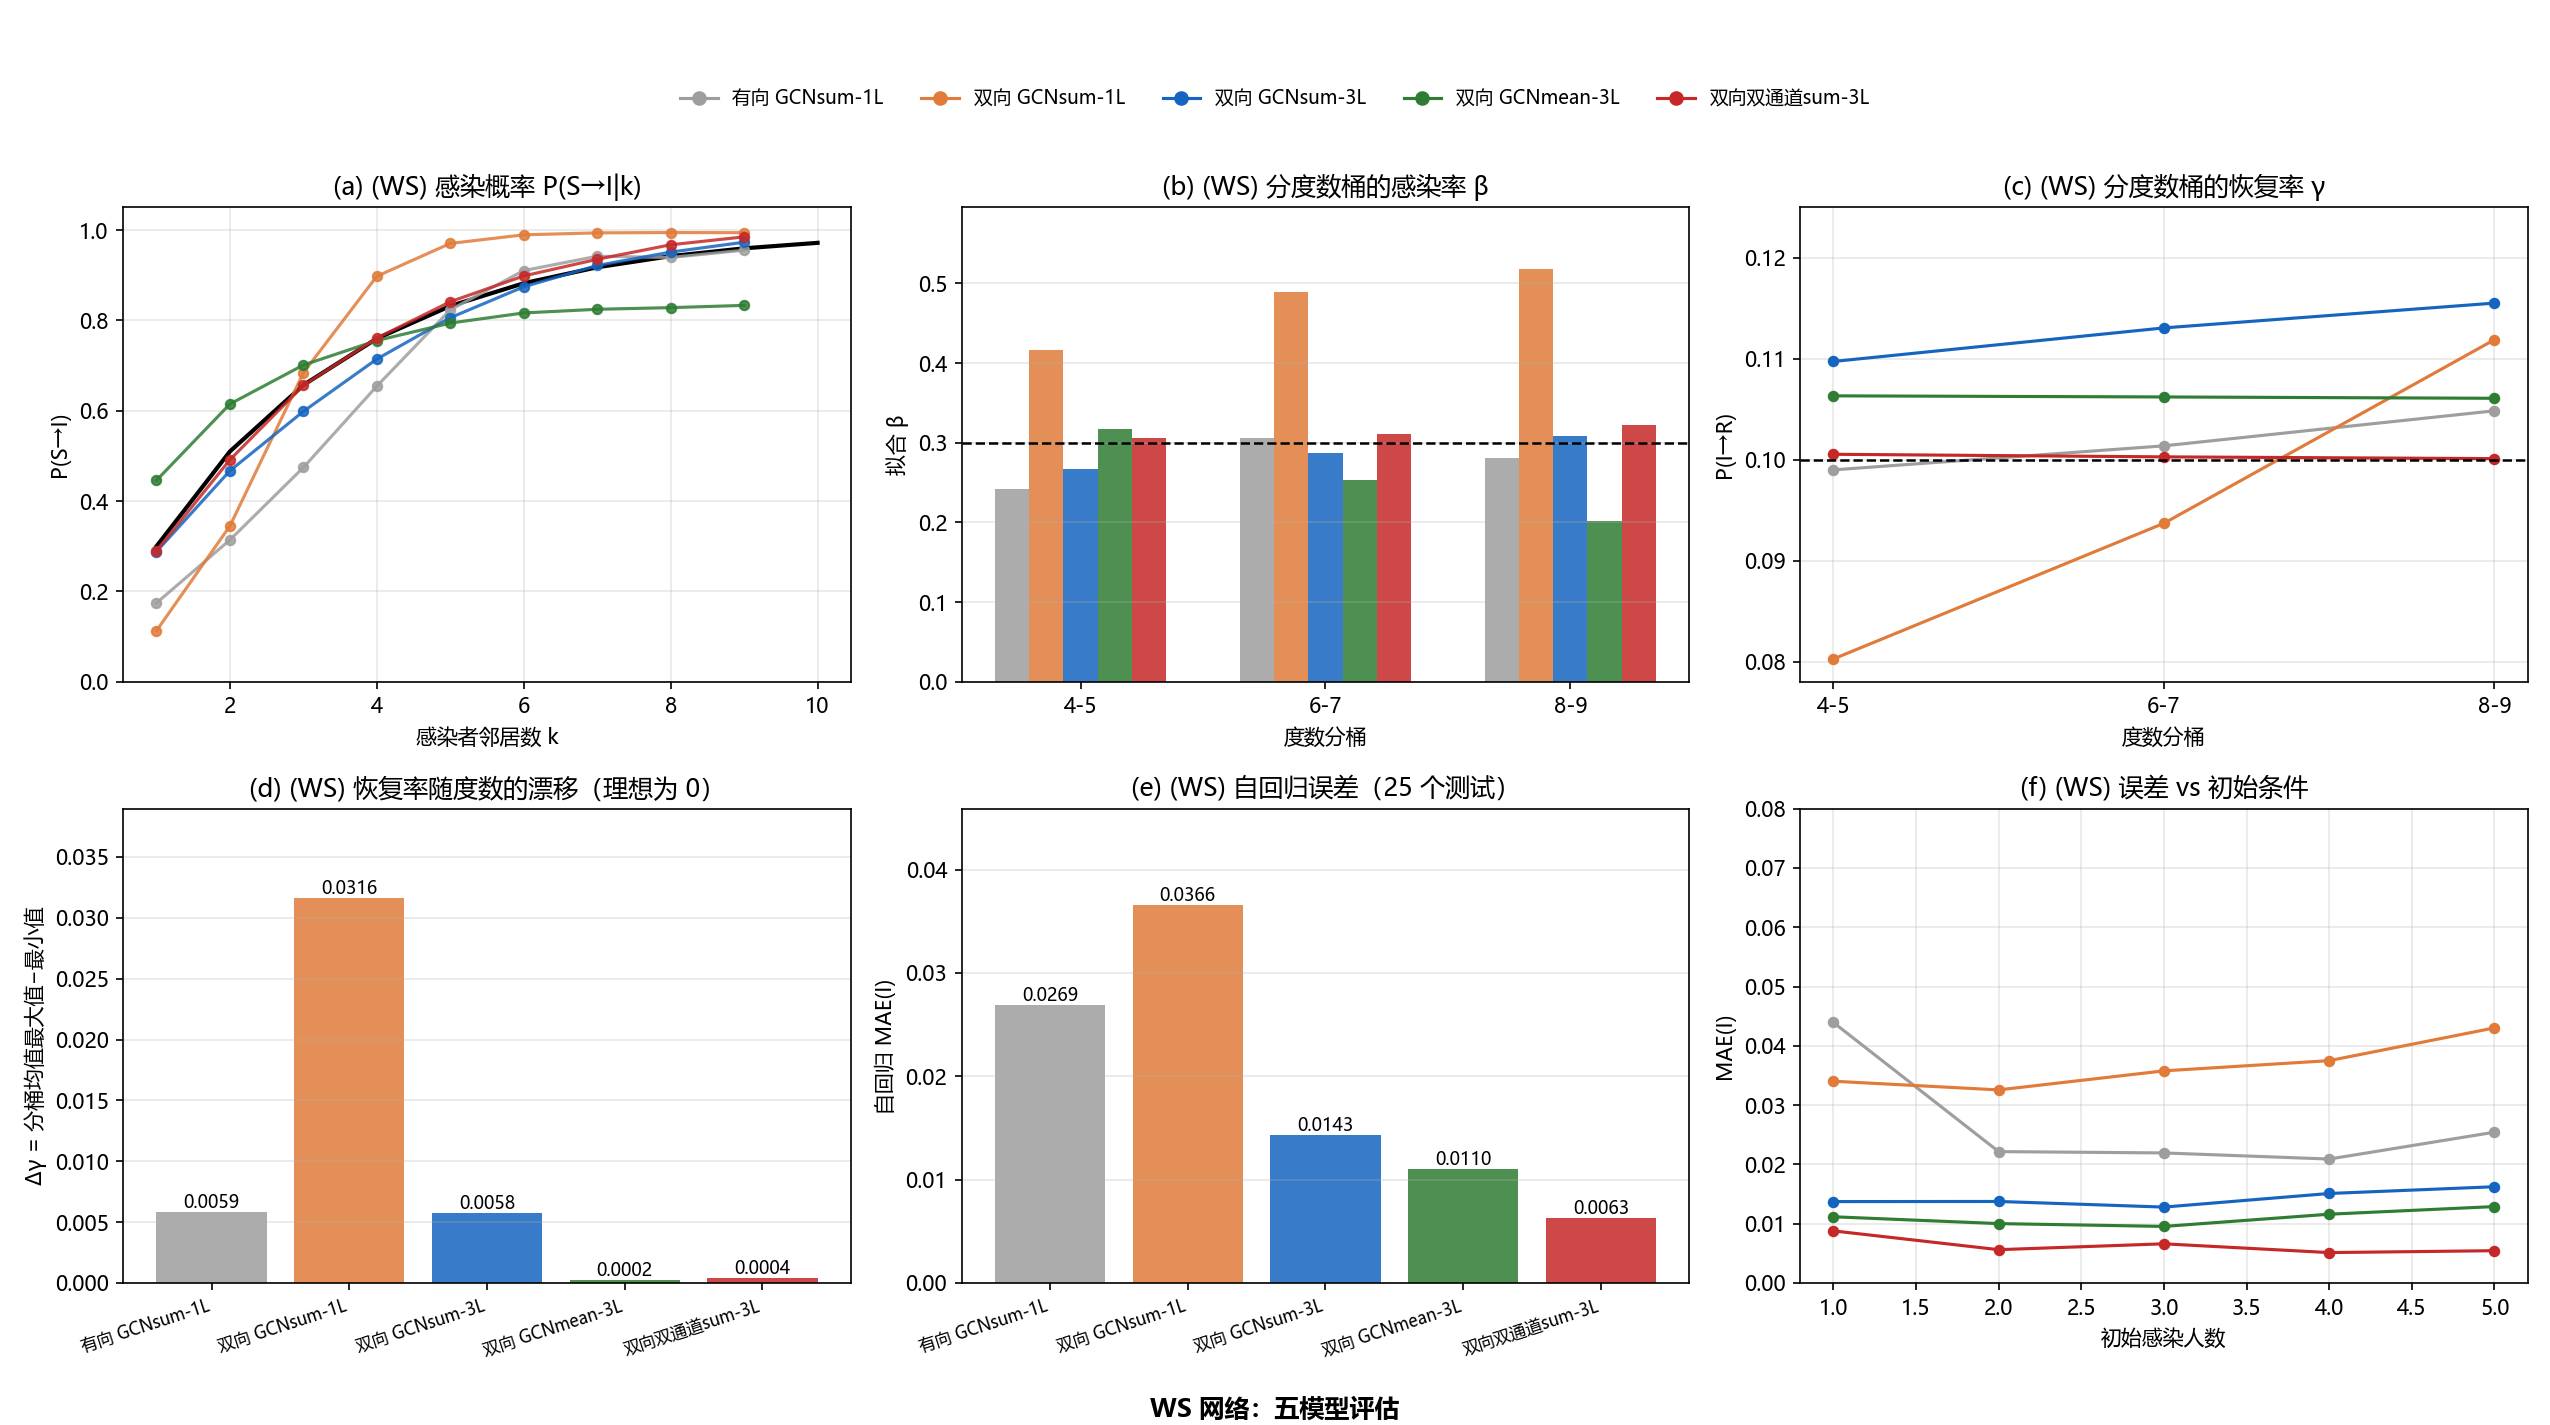
\includegraphics[width=0.96\linewidth]{fig_overview_WS.png}
  \caption{已知拓扑：WS 网络五模型完整诊断。}
\end{figure}
\end{landscape}

\begin{landscape}
\begin{figure}[p]
  \centering
  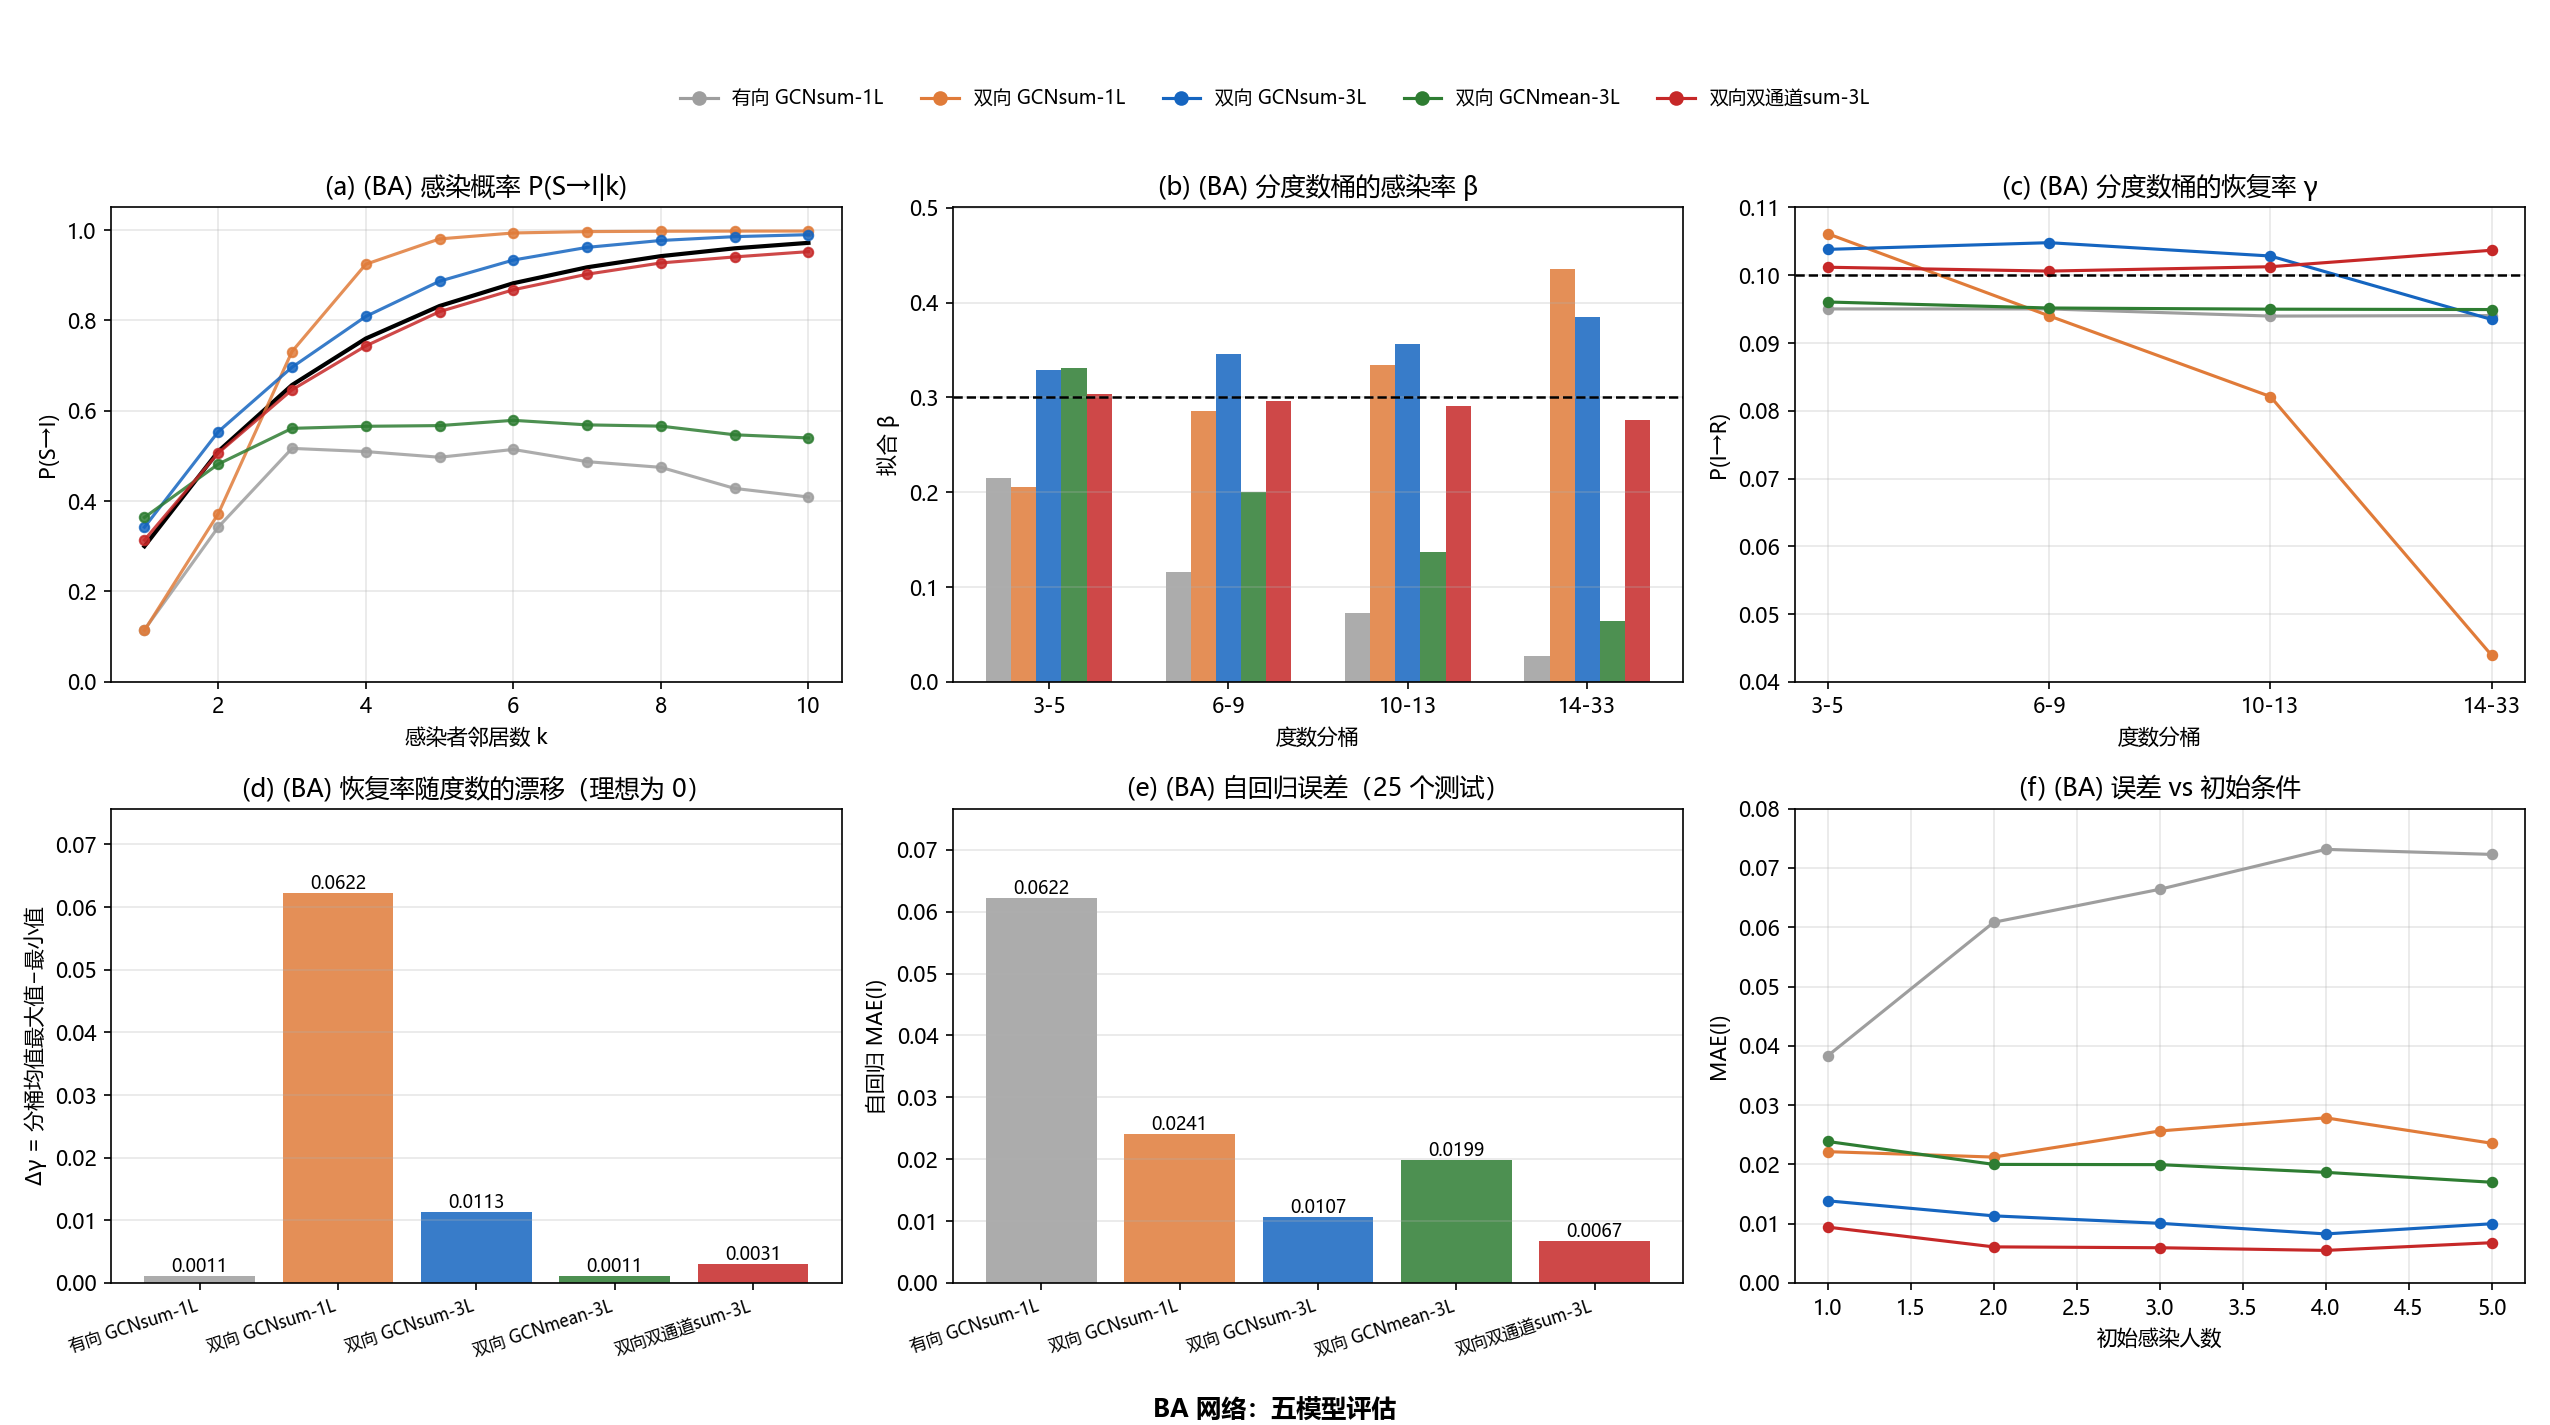
\includegraphics[width=0.96\linewidth]{fig_overview_BA.png}
  \caption{已知拓扑：BA 网络五模型完整诊断。}
\end{figure}
\end{landscape}

\subsection{未知拓扑完整诊断与训练曲线}

图\ref{fig:appendix-unknown-overview}给出未知拓扑所选模型的完整机制校准汇总，图\ref{fig:appendix-losses}给出三类网络的学习器损失、生成器损失、验证损失和温度轨迹。
训练曲线只能说明同分布状态对验证损失的变化，
不能据此判断轨迹级过拟合。

\begin{figure}[H]
  \centering
  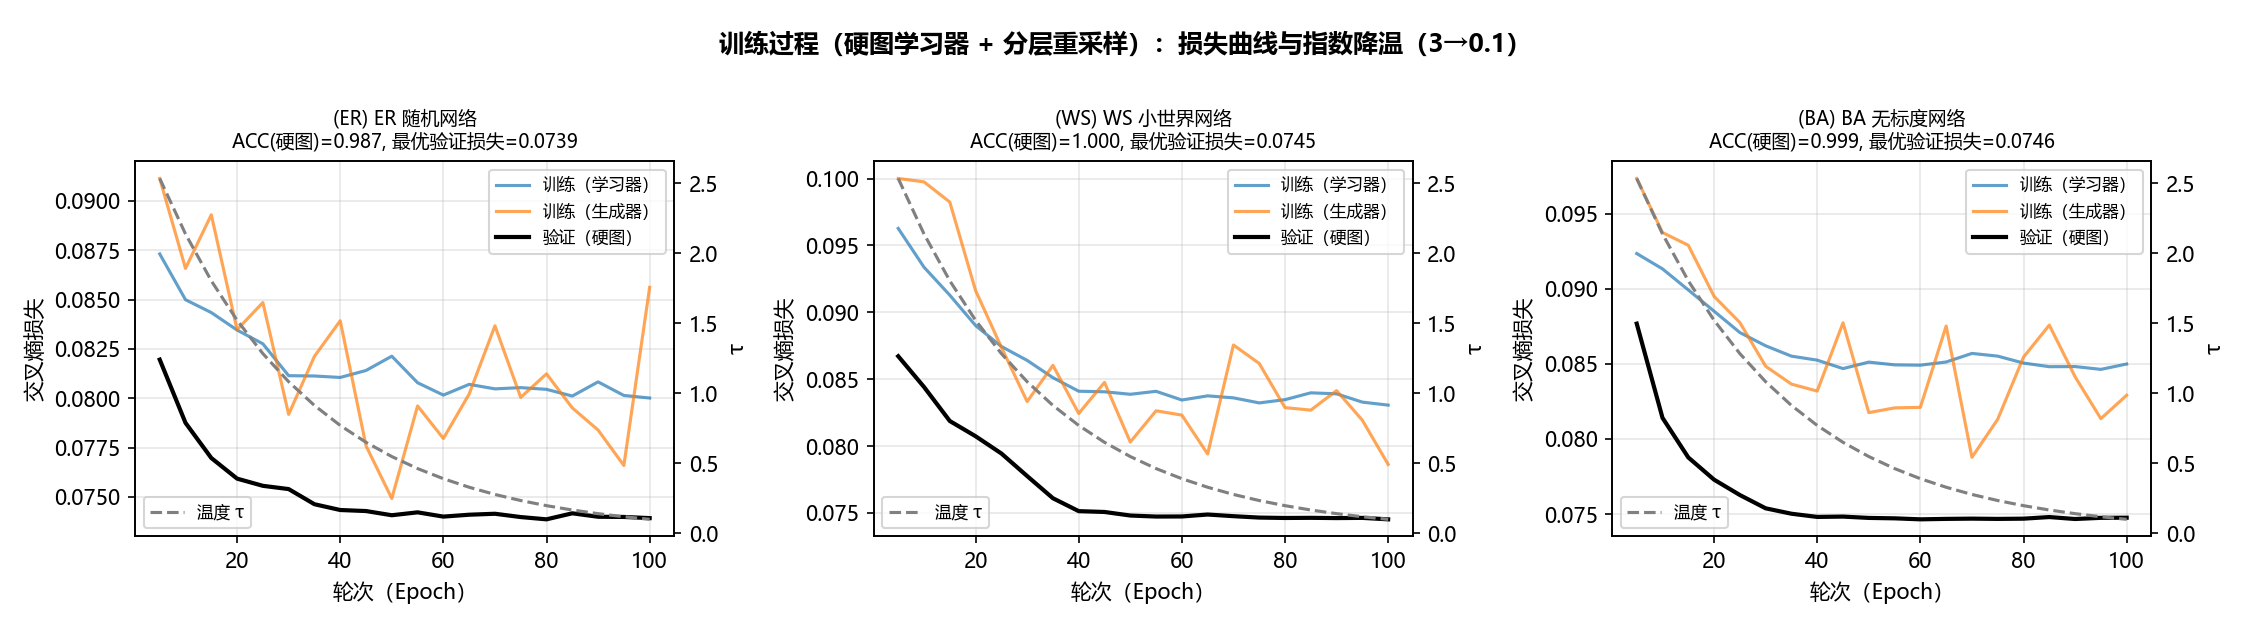
\includegraphics[width=\textwidth]{fig6_losses.png}
  \caption{未知拓扑：三个所选模型的训练损失、状态对级验证损失和温度变化。}
  \label{fig:appendix-losses}
\end{figure}

\begin{landscape}
\begin{figure}[p]
  \centering
  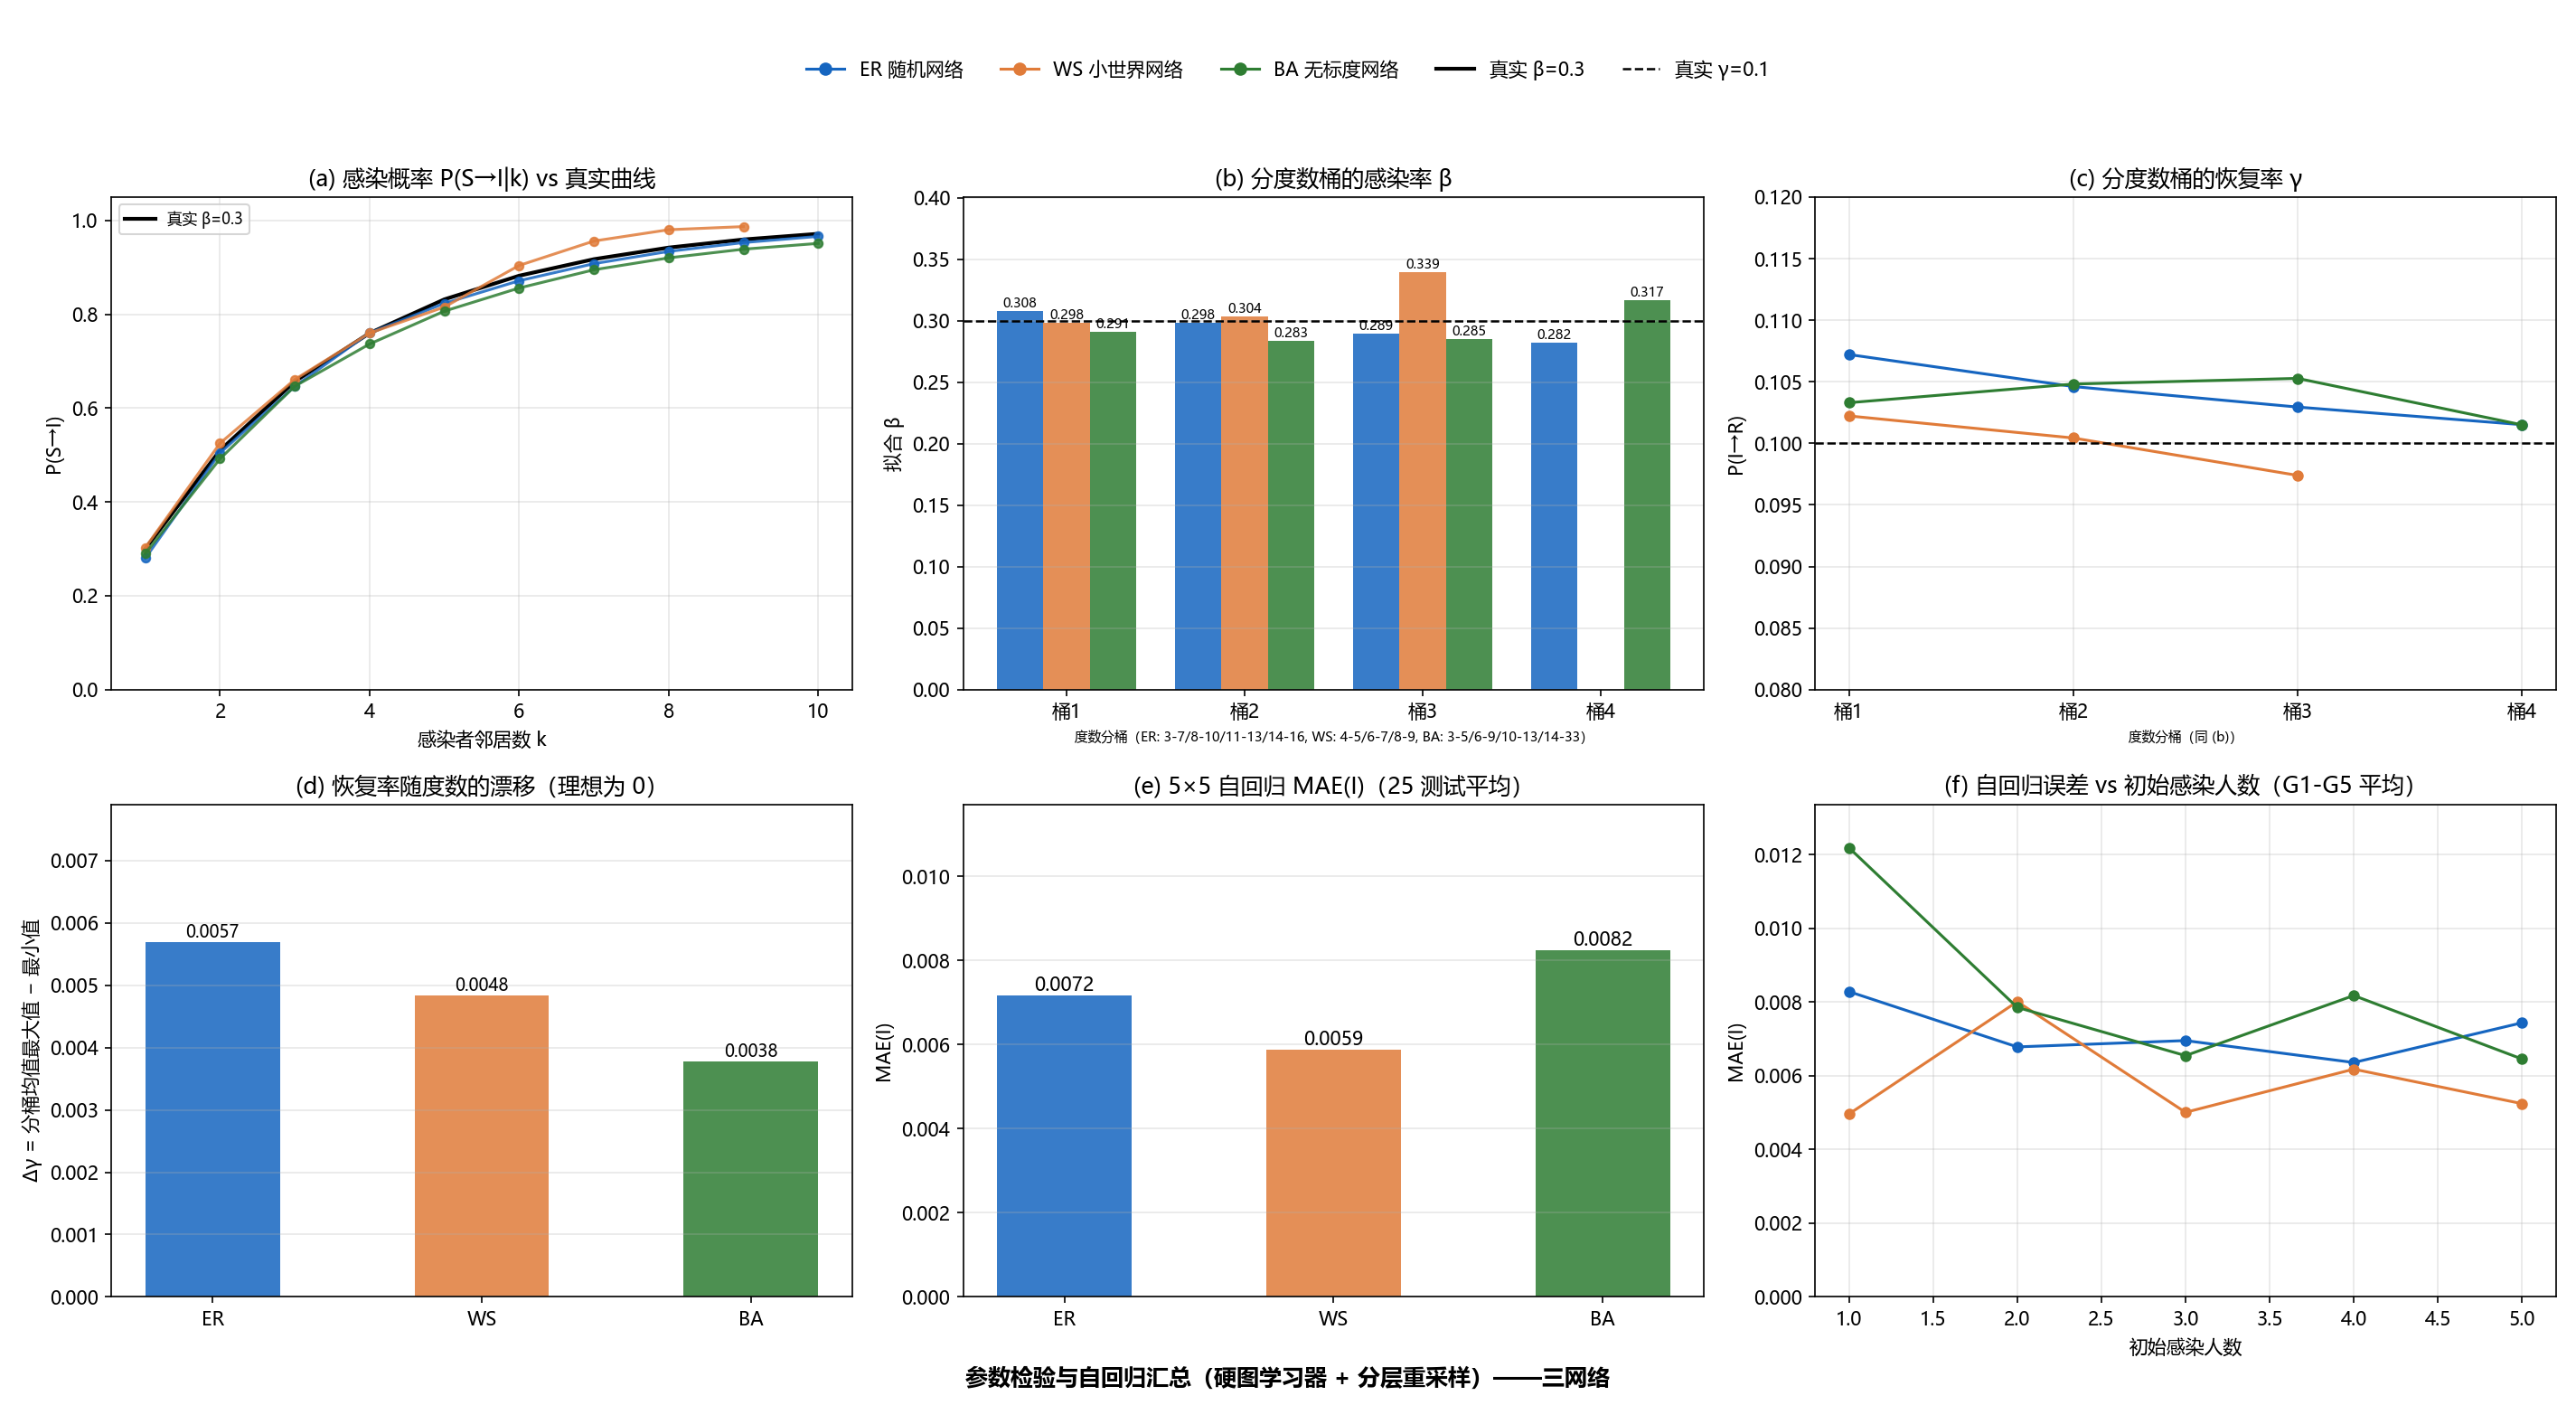
\includegraphics[width=0.96\linewidth]{fig6_overview_all.png}
  \caption{未知拓扑：所选 ER、WS、BA 模型的参数校准与自回归完整汇总。
正文数值从 JSON 重新读取，未直接从图中抄录。}
  \label{fig:appendix-unknown-overview}
\end{figure}
\end{landscape}

\clearpage
\subsection{完整 5×5 自回归网格}

图\ref{fig:appendix-autoreg-known-er}--图\ref{fig:appendix-autoreg-unknown-ba}保留所有自回归测试。
每张网格包含 5 组随机初始条件和 1--5 个初始感染者；
实线为真实模拟平均轨迹，
虚线为模型平均轨迹。
网格用于完整性核查，
正文只展示聚合误差和代表性平均曲线。

\begin{figure}[H]
  \centering
  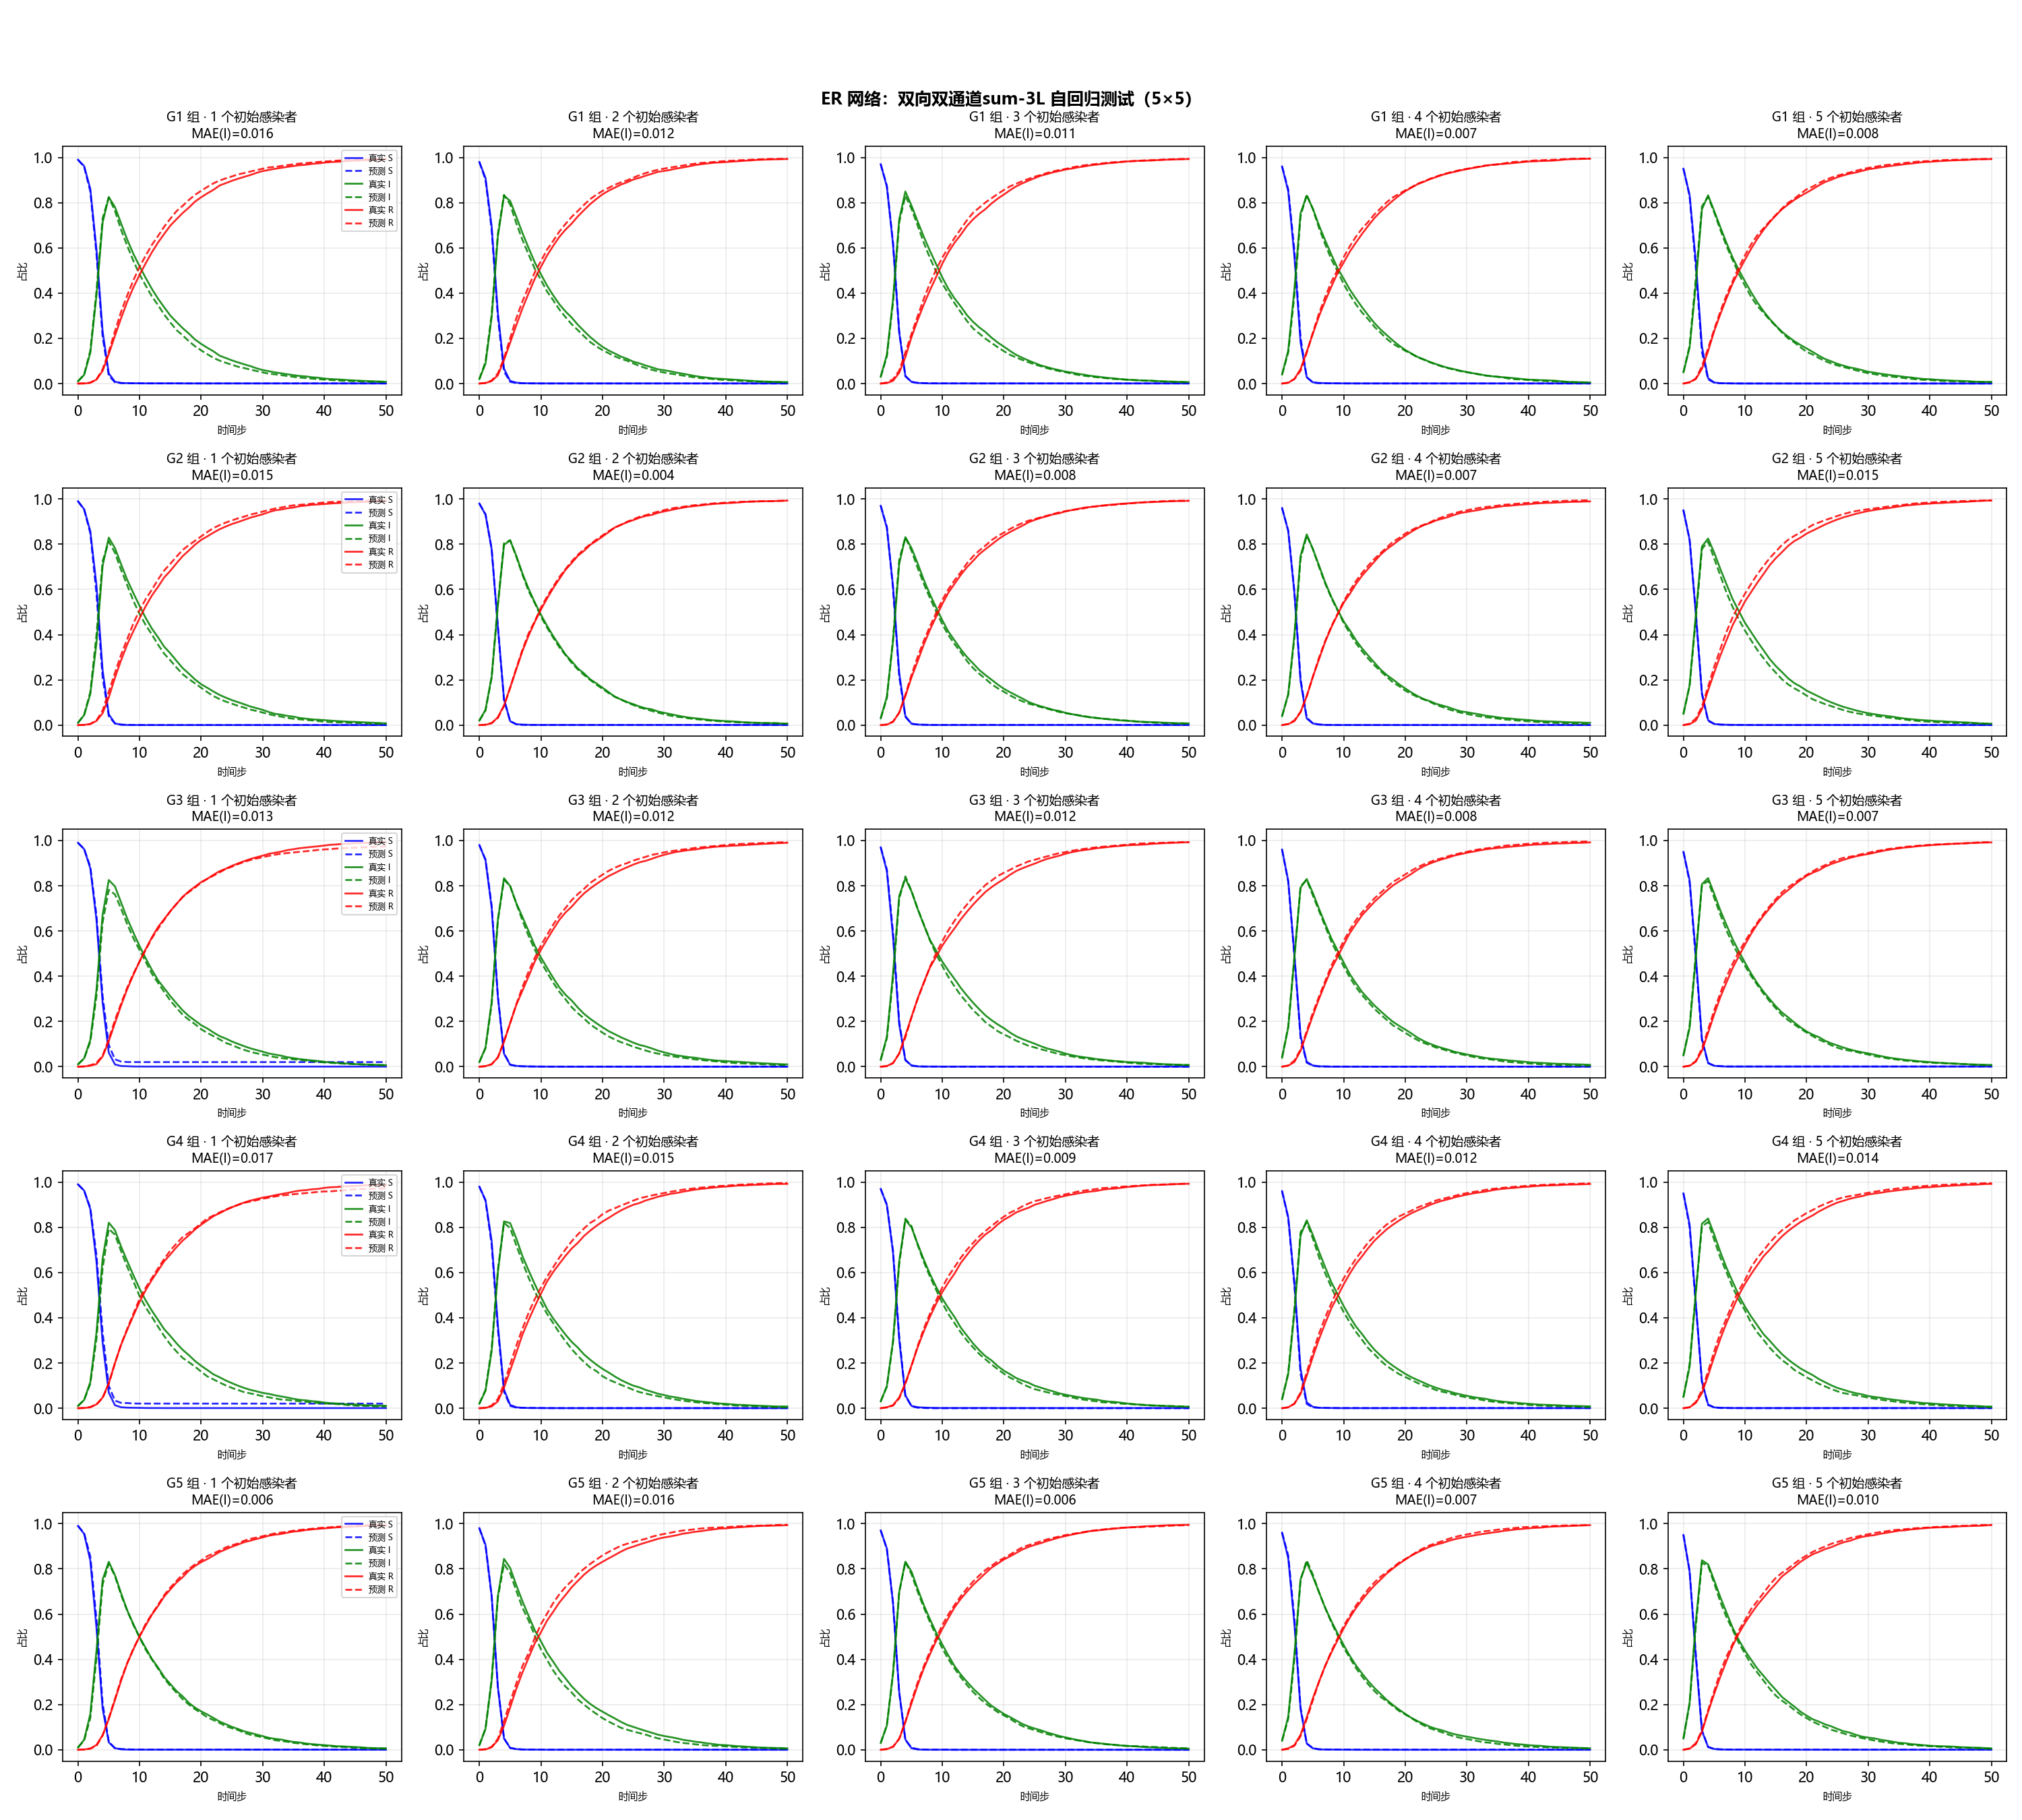
\includegraphics[width=0.95\textwidth]{fig_autoreg_grid_ER.png}
  \caption{已知拓扑双通道模型：ER 网络完整 5×5 自回归测试。}
  \label{fig:appendix-autoreg-known-er}
\end{figure}

\begin{landscape}
\begin{figure}[p]
  \centering
  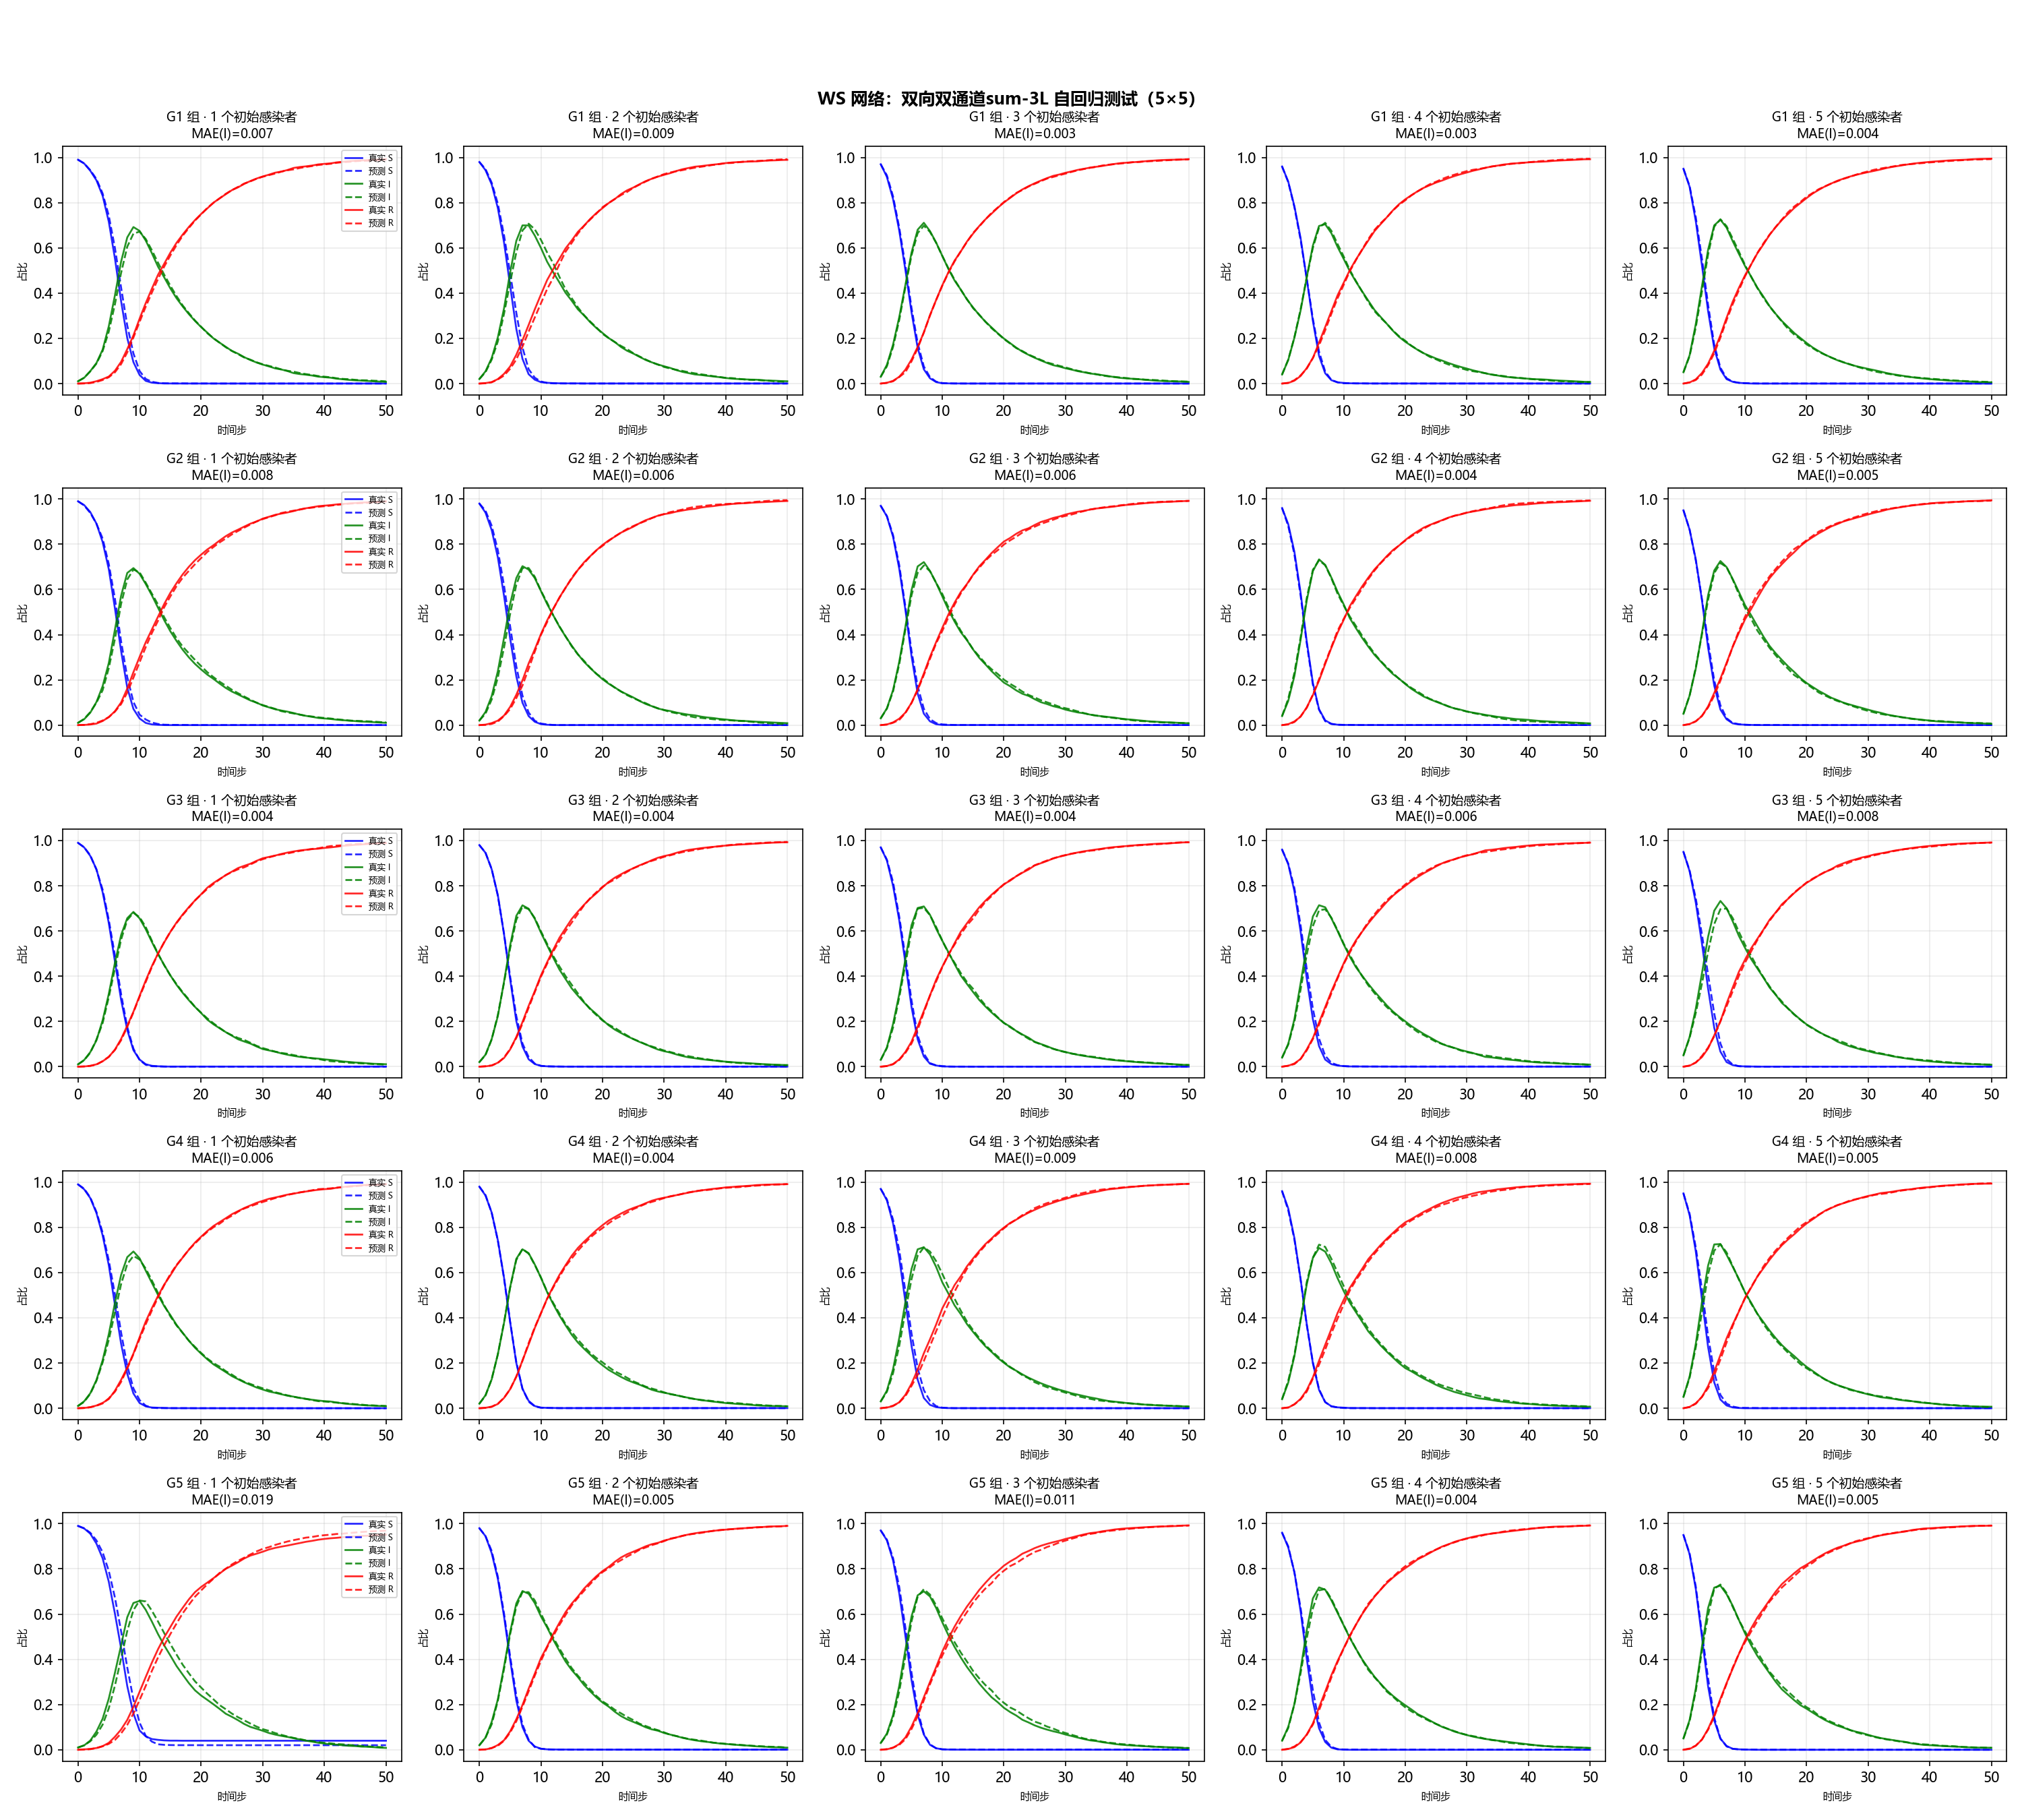
\includegraphics[height=0.86\textheight]{fig_autoreg_grid_WS.png}
  \caption{已知拓扑双通道模型：WS 网络完整 5×5 自回归测试。}
\end{figure}
\end{landscape}

\begin{landscape}
\begin{figure}[p]
  \centering
  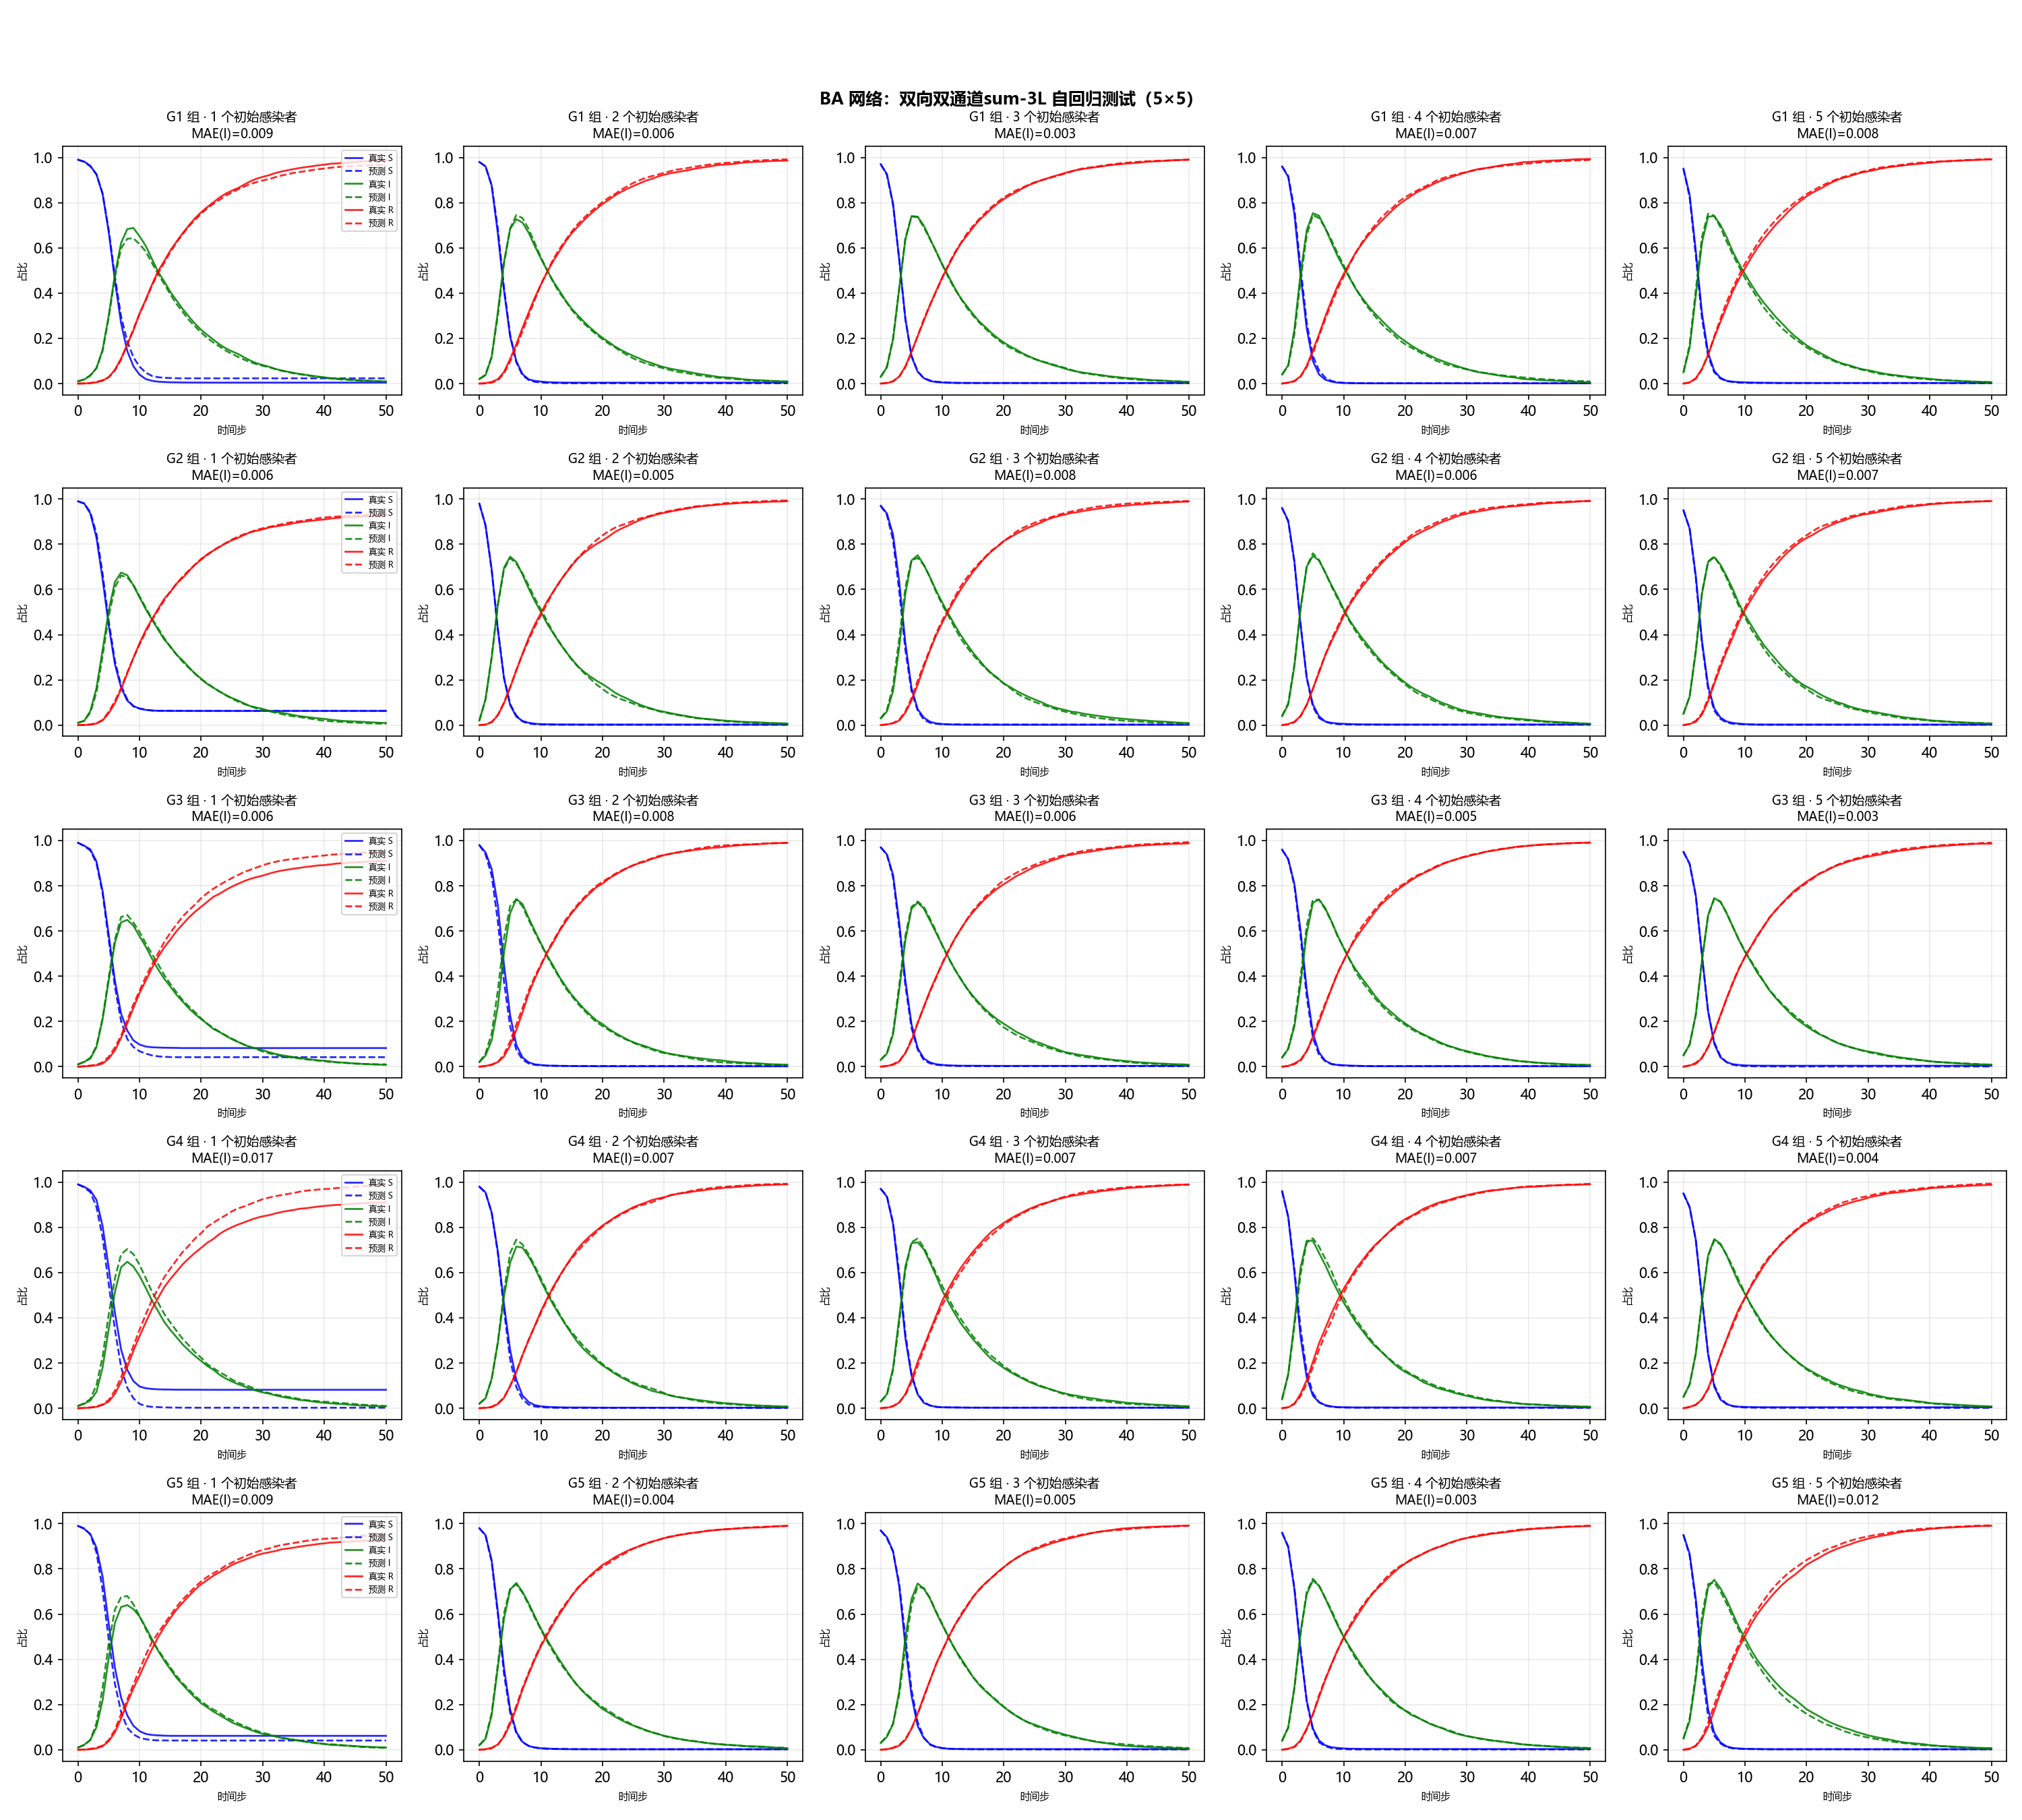
\includegraphics[height=0.86\textheight]{fig_autoreg_grid_BA.png}
  \caption{已知拓扑双通道模型：BA 网络完整 5×5 自回归测试。}
\end{figure}
\end{landscape}

\begin{landscape}
\begin{figure}[p]
  \centering
  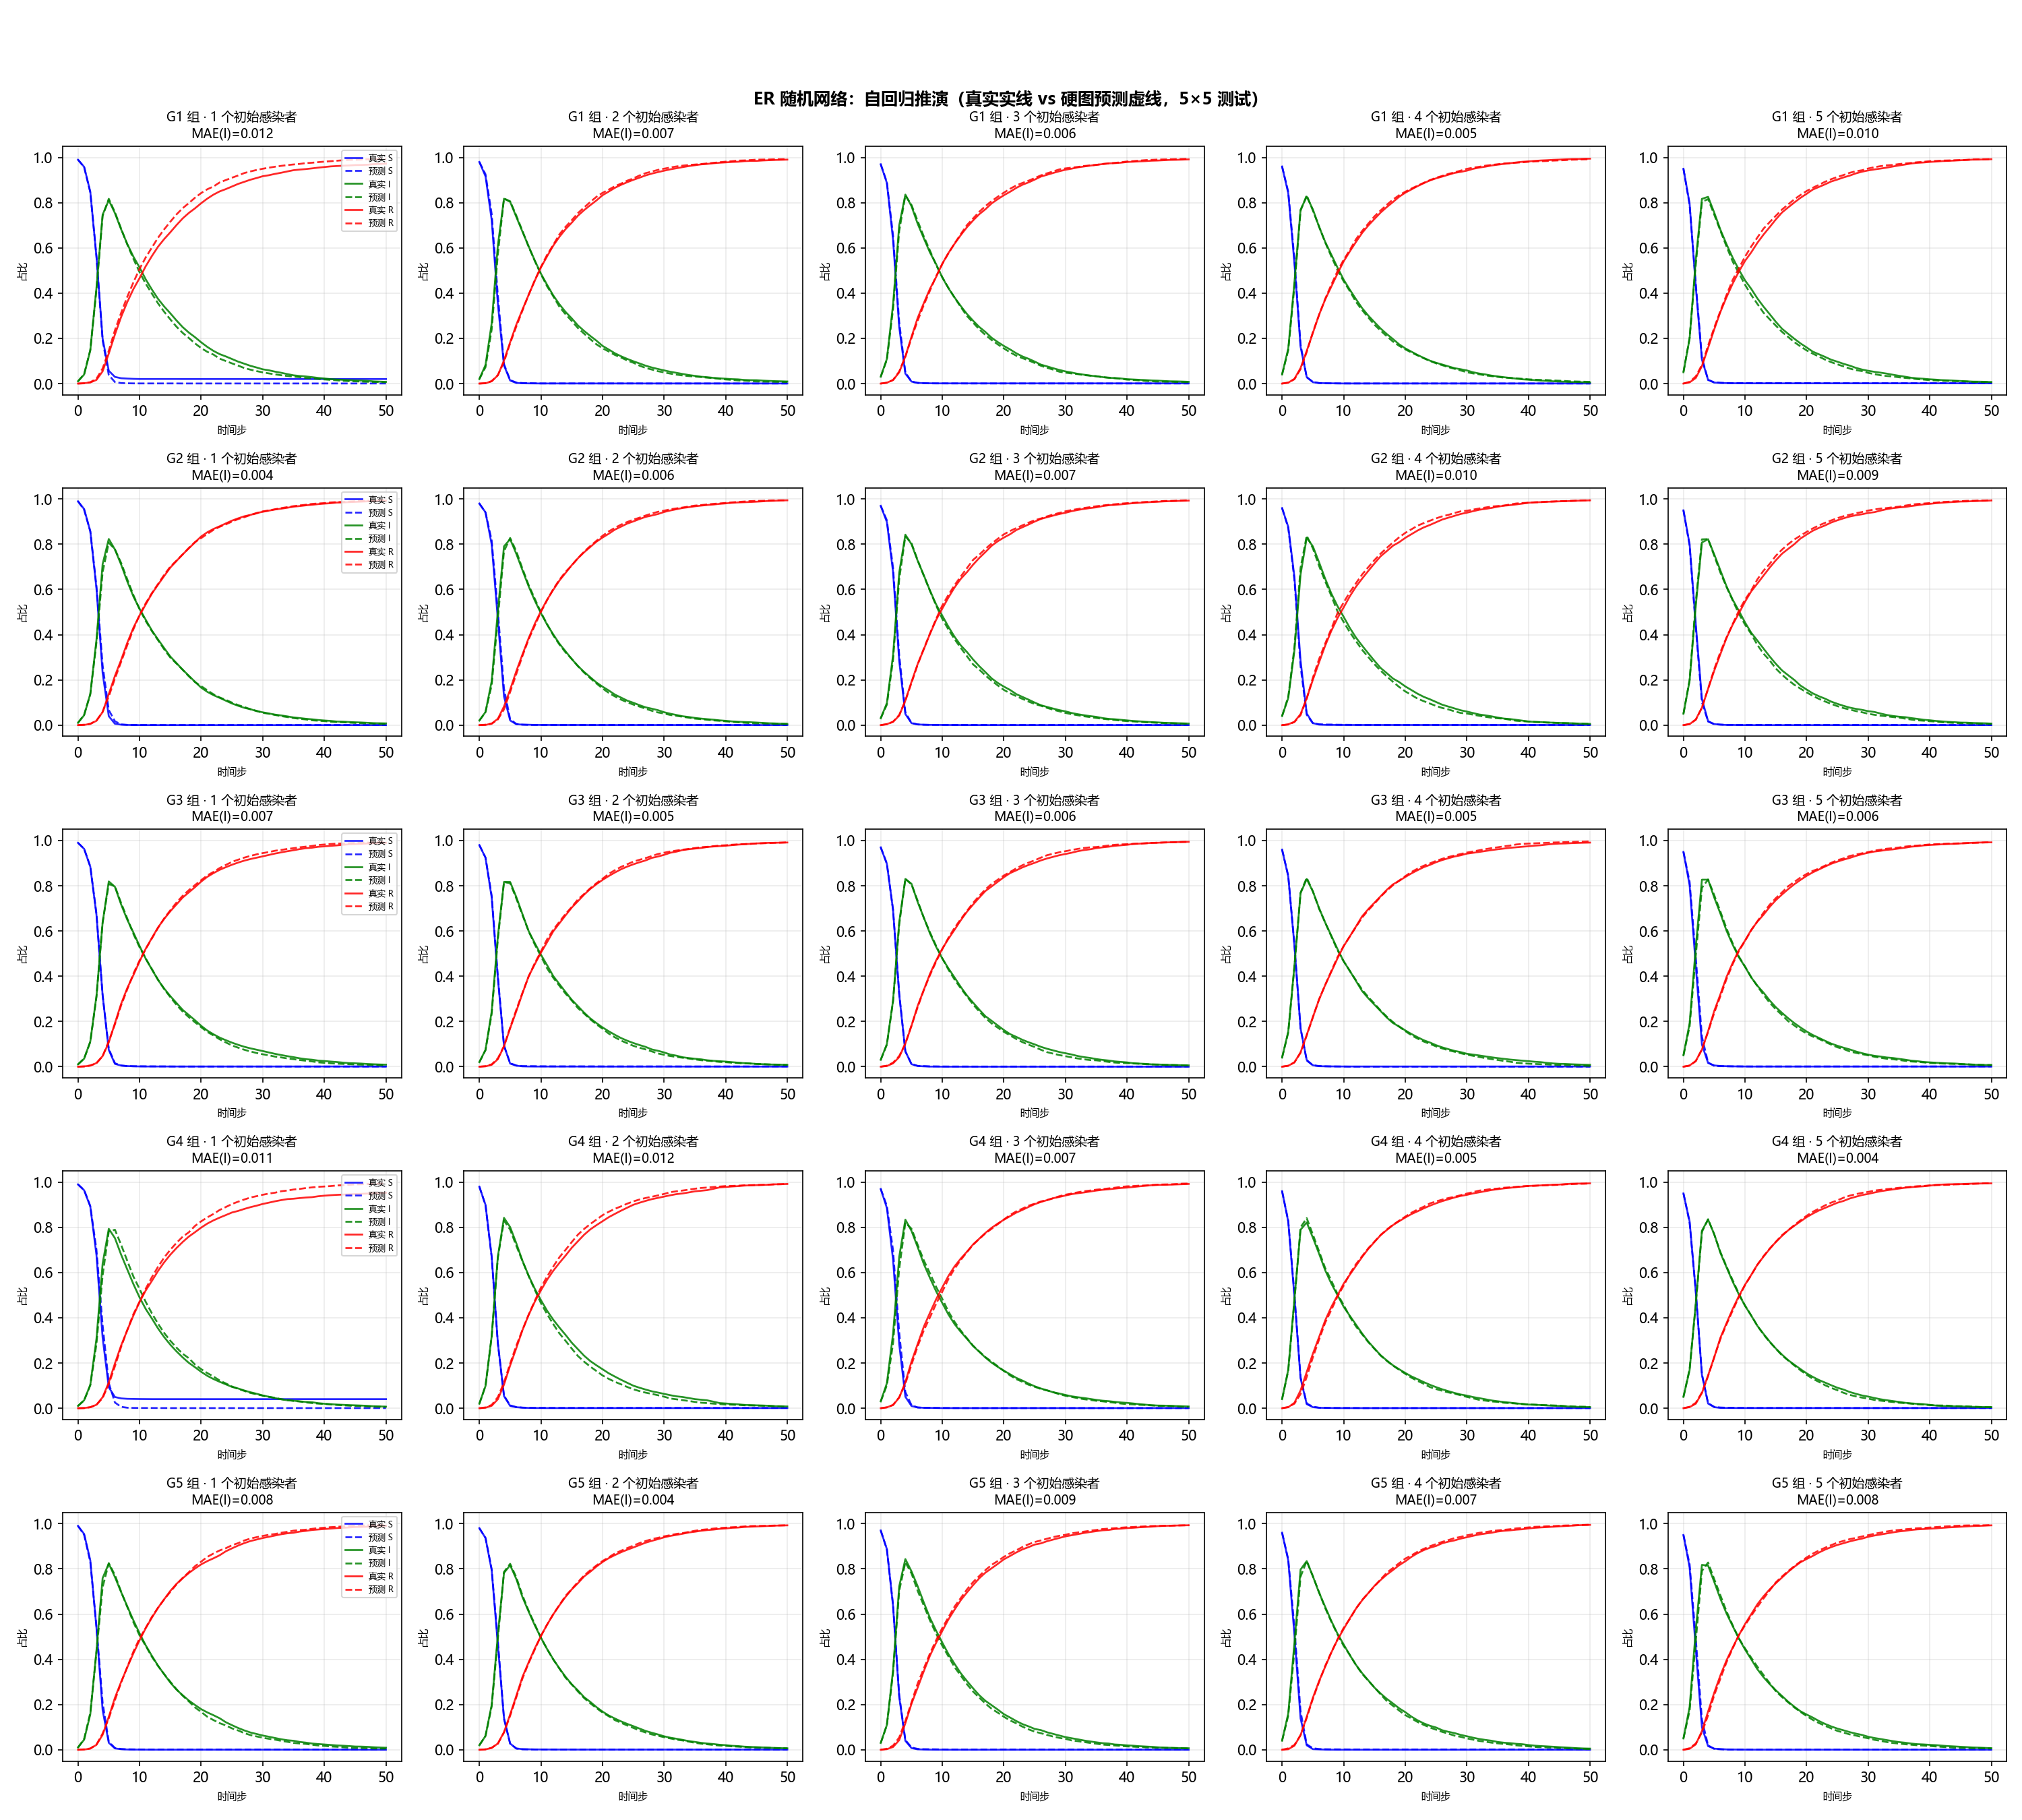
\includegraphics[height=0.86\textheight]{fig6_autoreg_grid_ER.png}
  \caption{未知拓扑所选模型：ER 网络完整 5×5 自回归测试。}
\end{figure}
\end{landscape}

\begin{landscape}
\begin{figure}[p]
  \centering
  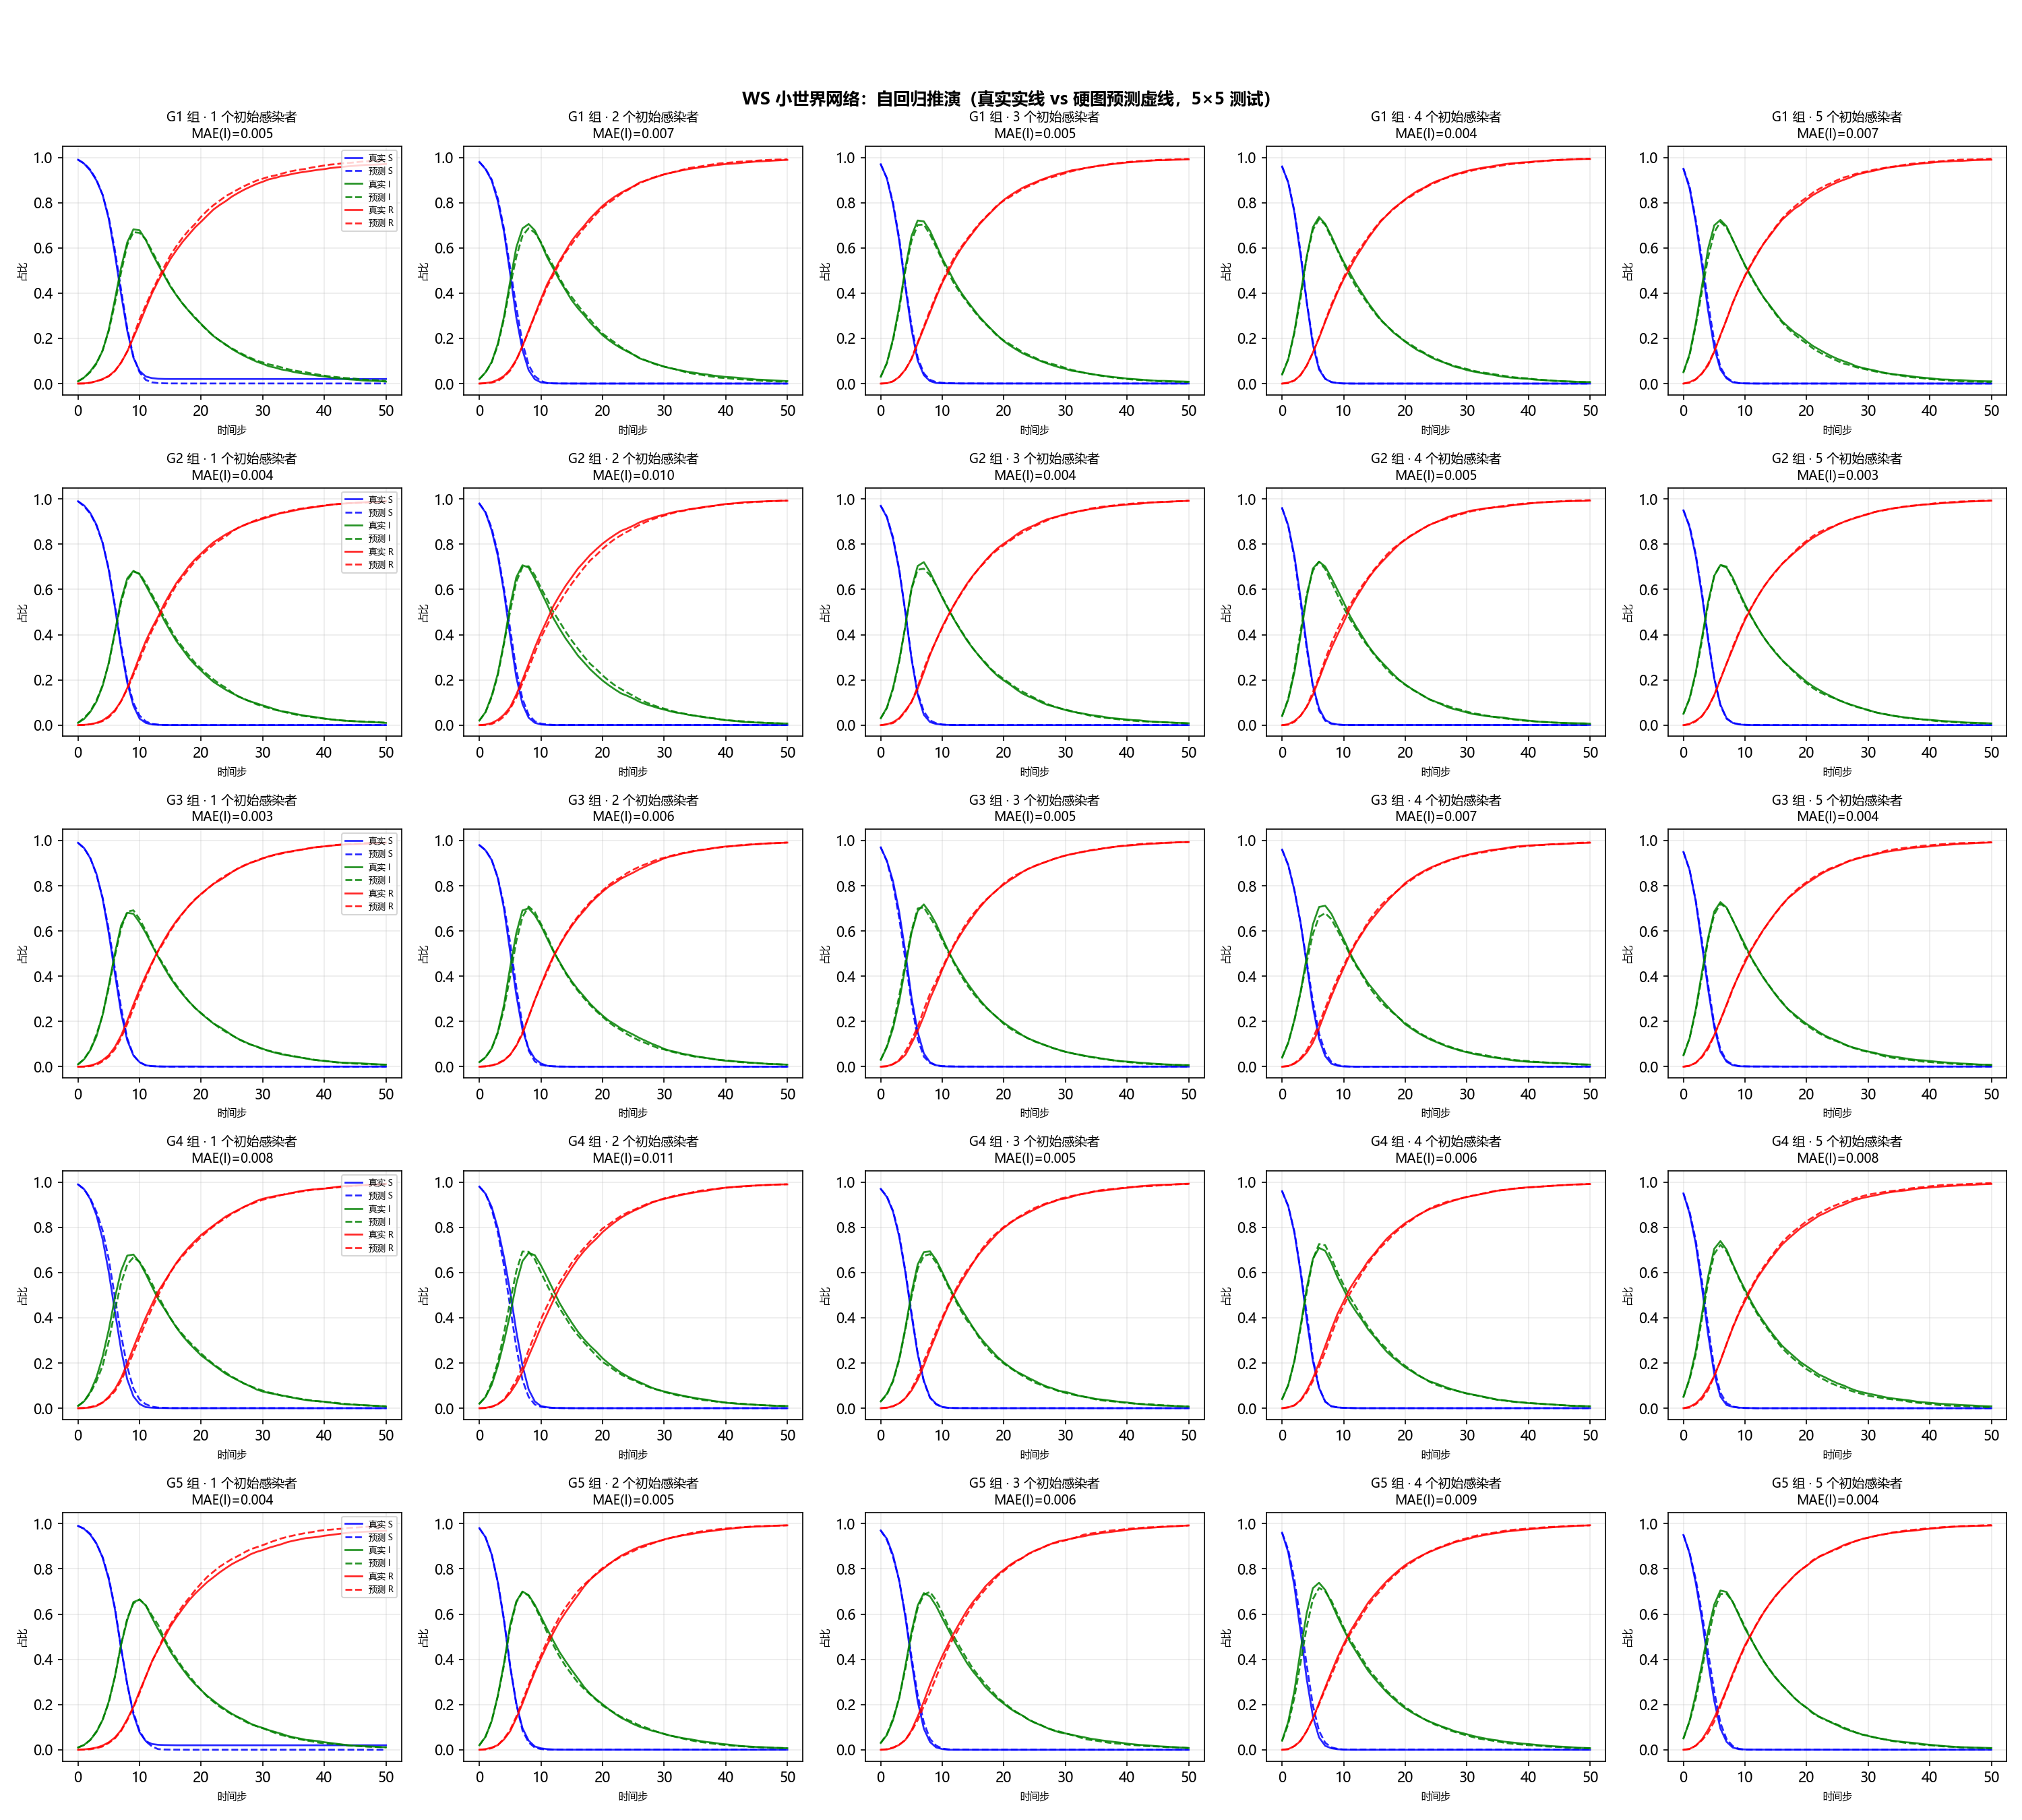
\includegraphics[height=0.86\textheight]{fig6_autoreg_grid_WS.png}
  \caption{未知拓扑所选模型：WS 网络完整 5×5 自回归测试。}
\end{figure}
\end{landscape}

\begin{landscape}
\begin{figure}[p]
  \centering
  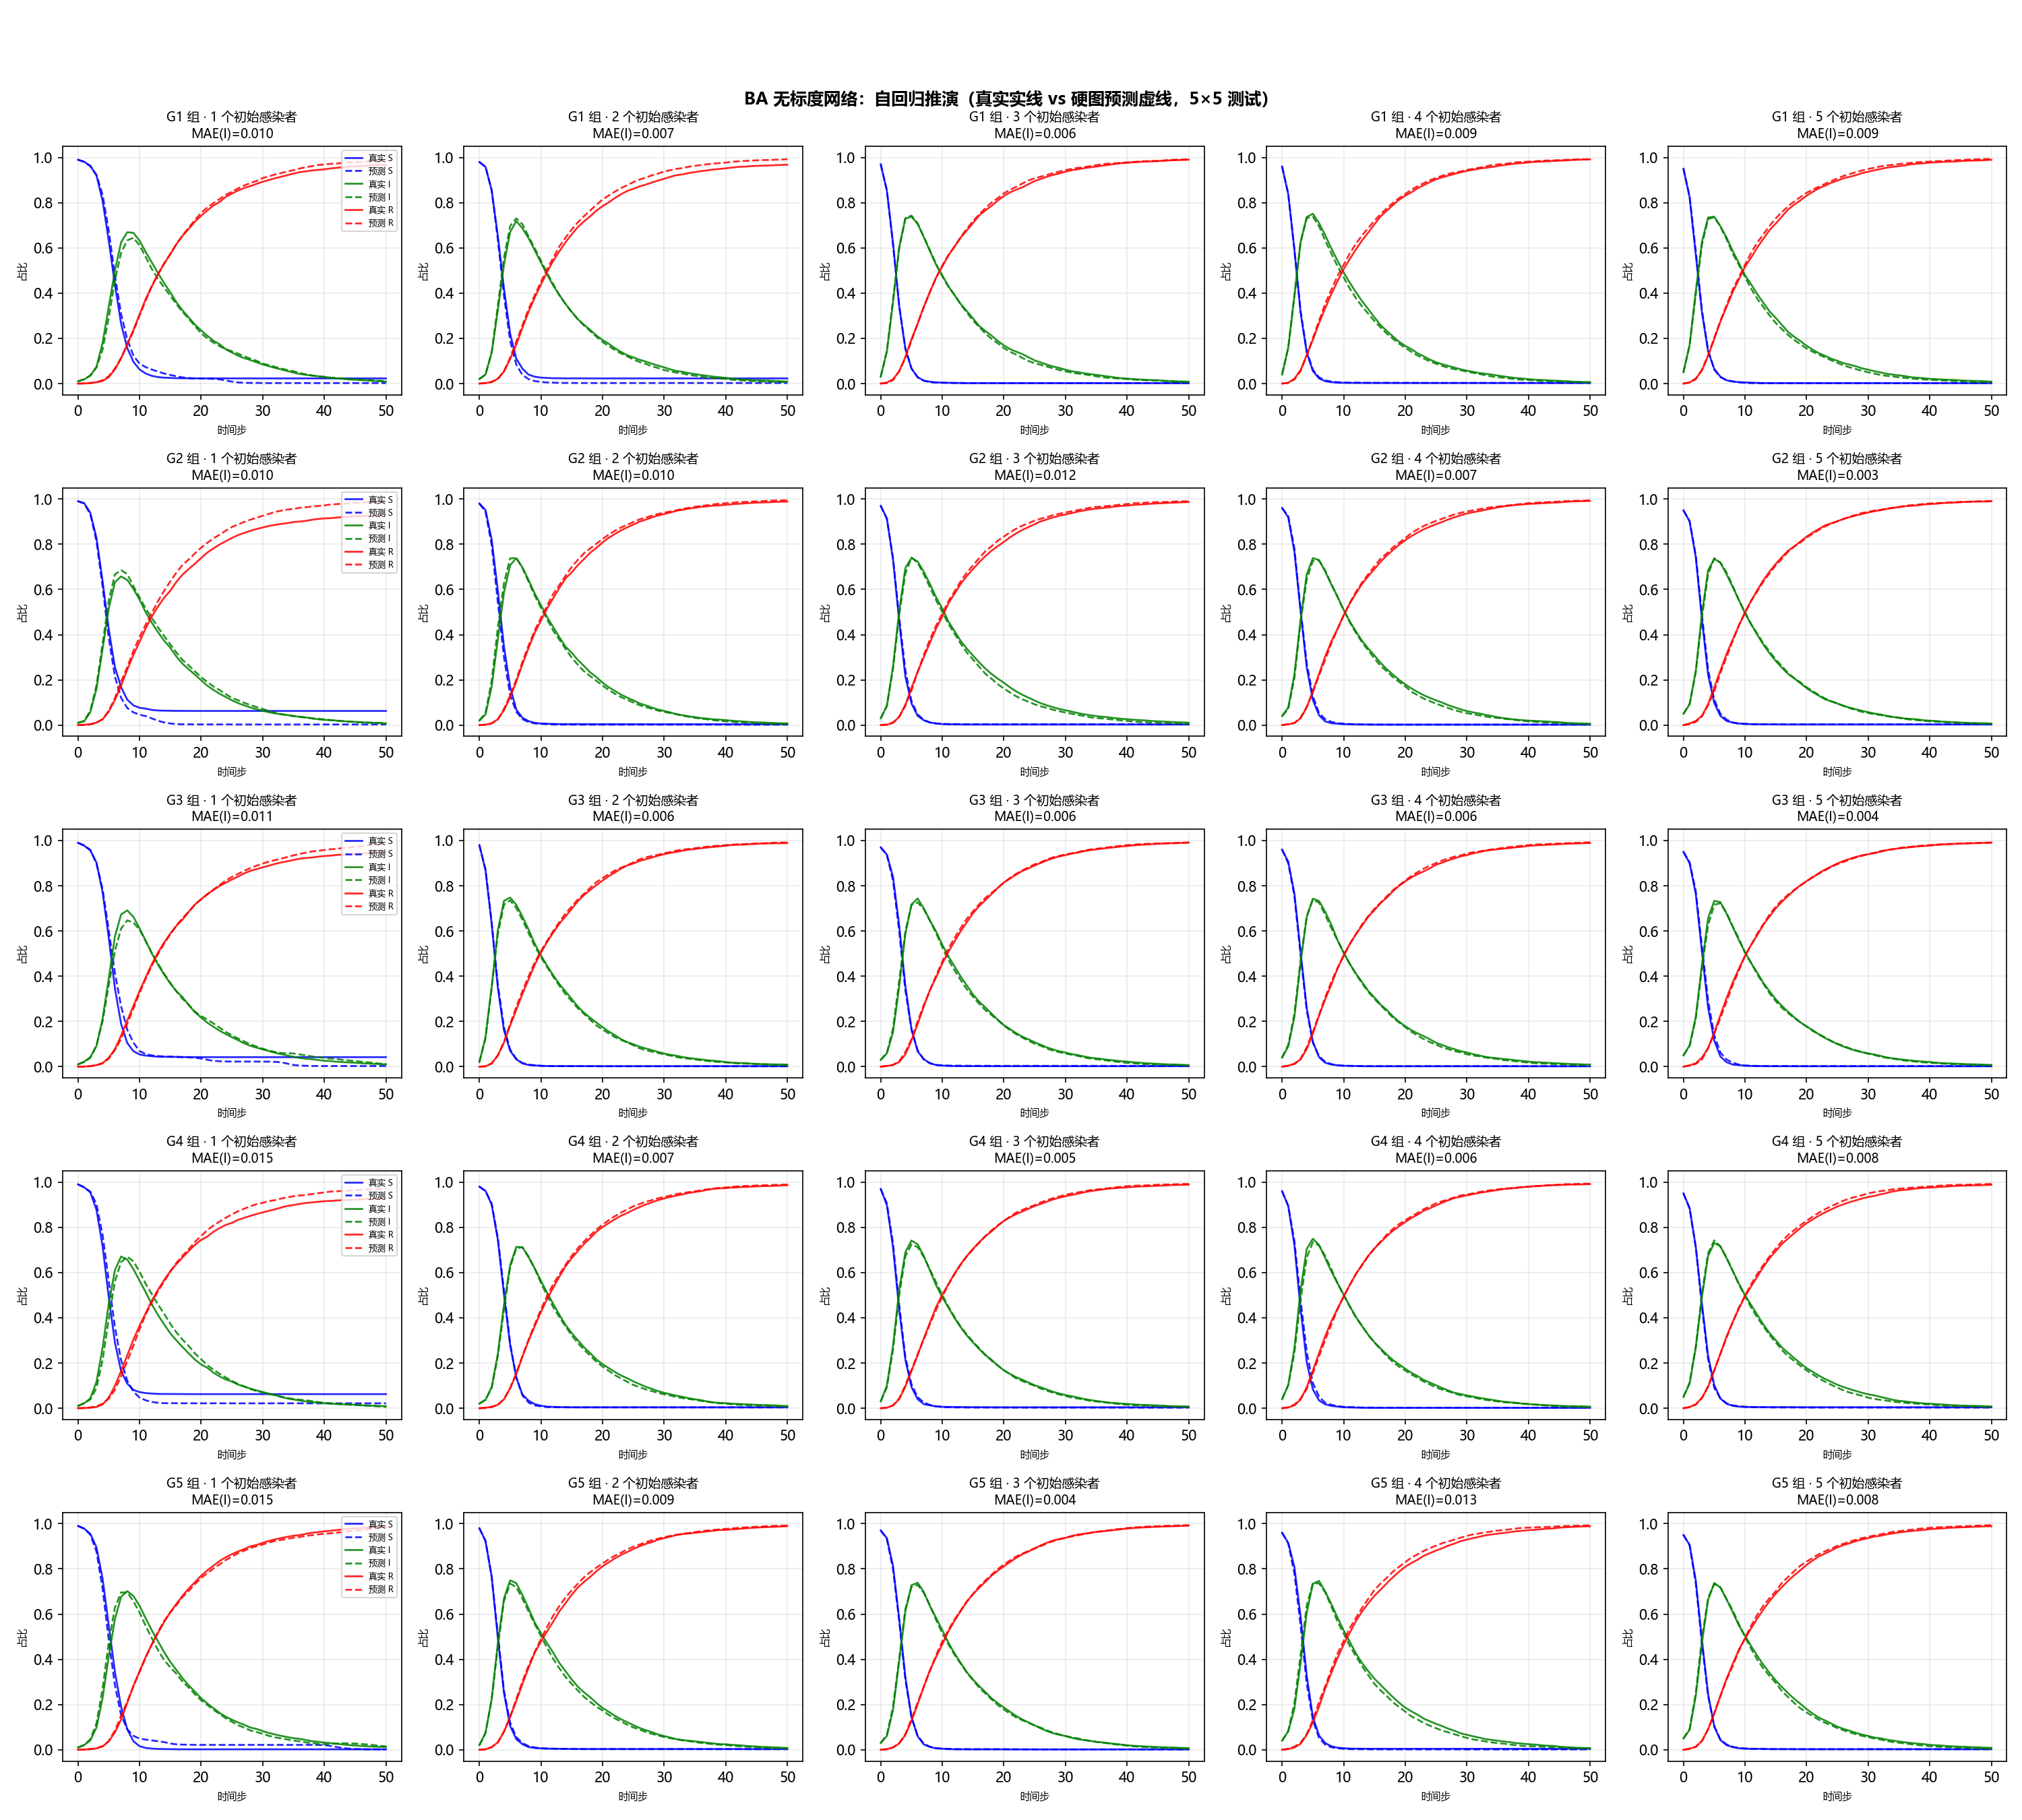
\includegraphics[height=0.86\textheight]{fig6_autoreg_grid_BA.png}
  \caption{未知拓扑所选模型：BA 网络完整 5×5 自回归测试。}
  \label{fig:appendix-autoreg-unknown-ba}
\end{figure}
\end{landscape}

\clearpage
\subsection{探索性失败实验汇总}

表\ref{tab:negative-results}汇总能够从保存 JSON 直接追溯的主要负结果。
不同配置之间不满足严格单变量条件，
因此这些数字只说明“在相应 BA 实例与配置下未改善”，
而不支持普遍方法定律。

\begin{table}[H]
  \centering
  \caption{未知拓扑开发阶段的探索性结果。}
  \label{tab:negative-results}
  \begin{tabularx}{0.92\textwidth}{@{}lXr@{}}
    \toprule
    网络/方案 & 说明 & 硬图 ACC \\
    \midrule
    ER 基础硬图版 & phase6 basic & 0.908 \\
    WS 基础硬图版 & phase6 basic & 0.998 \\
    BA 基础硬图版 & phase6 basic & 0.818 \\
    BA 两阶段版 & 软图粗学后硬图精修 & 0.888 \\
    BA 闭环多步 $P=2$ & 离散状态闭环回馈 & 0.562 \\
    BA 闭环多步 $P=3$ & 离散状态闭环回馈 & 0.299 \\
    BA teacher-forcing $P=2$ & 真实中间状态回馈 & 0.578 \\
    BA teacher-forcing $P=3$ & 真实中间状态回馈 & 0.496 \\
    \bottomrule
  \end{tabularx}
\end{table}

\section{复现文件与软件环境}

\subsection{来源文件}

正文数值的唯一实验来源如下：
\begin{itemize}
  \item \nolinkurl{two_channel_experiment/results/phase4/phase4_five_models.json}；
  \item \nolinkurl{two_channel_experiment/results/phase6/dgsl_l1b_ER.json}、\nolinkurl{WS.json}、\nolinkurl{BA.json}；
  \item phase6 中 ER/WS/BA 各 seed 7、21、42 的九个逐 seed JSON。
\end{itemize}
\nolinkurl{paper/notebooks/} 中的两份 notebook 分别生成三张方法图和三张结果图，
并由结果绘图 notebook 生成 \nolinkurl{metrics_manifest.json}。
\nolinkurl{paper/scripts/build_figures.py} 为统一执行入口。
清单包含全部来源 SHA-256、派生 Precision/F1、跨网络平均指标及选中模型。
\nolinkurl{paper/scripts/verify_results.py} 再次核对哈希、phase4 关键数值、最低验证 CE 选模规则和 phase6 边数。

\subsection{软件版本}

实验环境经实际虚拟环境核对为：Python 3.13.7、PyTorch 2.12.0+cpu\cite{paszke2019}、PyTorch Geometric 2.7.0\cite{fey2019}、NetworkX 3.5\cite{hagberg2008}、NumPy 2.2.6、SciPy 1.16.2、Matplotlib 3.10.6，
优化器使用 Adam\cite{kingma2015adam}。
未知拓扑实现参考 GGN 官方代码的交替训练语义\cite{ggncode}。
论文使用 TeX Live 2025、XeLaTeX、latexmk 4.87 和 biber 2.21 编译；
PDF 使用 Poppler 26.07 渲染检查。

\subsection{结果解释约定}

为避免常见误读，复现时采用以下约定：
\begin{enumerate}
  \item “5×5”指 5 组评估初始条件与 1--5 个初始感染者，不是 5 个训练 seed；
  \item $\hat\gamma\pm s$ 中的 $s$ 是控制状态上的输出离散度，不是置信区间；
  \item phase4 的最终结果已使用修复后的 SIR 邻接去重模拟器；
phase0/phase1 的旧自回归数值不纳入正文；
  \item 未知拓扑的 data seed 固定为 21，train seed 为 7、21、42；
训练 seed 的变化不得触发重新生成真实图；
  \item 若修改网络、$\beta$、$\gamma$ 或 $T$，必须同时更新缓存键或删除旧缓存，不能无条件复用 \code{data\_ER.npz} 等文件。
\end{enumerate}
